\documentclass[TA.tex]{subfiles}

\begin{document}


%\hyphenation{equi-va-len-cia}\hyphenation{pro-pie-dad}\hyphenation{res-pec-ti-va-men-te}\hyphenation{sub-es-pa-cio}

\chapter{Homología}

Para nociones de homología simplicial, consultar los apuntes de Homología Simplicial. Atención: en homología ordenada no existen los símplices en orden distinto al prefijado, no se toma cociente. 
\section{Homología singular}

Dado un espacio topológico $X$, definimos un $n$-\emph{símplice singular} como una aplicación continua $\sigma_n:\Delta^n\to X$, donde $\Delta^n$ es el $n$-símplice estándar. Denotamos $C_n(X)$ al grupo abeliano libre de todos los $n$-símplices singulares. A las combinaciones de la forma $\sum_{i=1}^n\lambda_i\sigma_n^i$ con $\lambda_i\in\Z$ se las llama $n$-\emph{cadenas} (estos son de hecho todos los elementos de $C_n(X)$. Tenemos definido también el operador borde $d_n:C_n(X)\to C_{n-1}(X)$, que es un homomorfismo de grupos abelianos definido como $d_n(\sigma_n)=\sum_{i=0}^n \sigma_n|_{[v_0,\dots, \hat{v_i},\dots, v_n]}$. Este operador verifica las mismas propiedades que el operador borde entre complejos simpliciales, con idéntica demostración. Así que hemos construido un complejo de cadenas singulares $\{C_n(X), d_n\}_{n\geq 1}=C_*(X)$. En caso de usar coeficientes en un grupo $G$ se indicará como $C_*(X,G)$. Análogamente a la homología simplicial, si $z\in C_n(X)$ y $d(z)=0$, decimos que $z$ es un $n$-ciclo. Si $z=d_{n+1}(z')$ para algún $z'\in C_{n+1}(X)$, decimos que $z$ es un $n$-borde. Como tenemos $B_n(X)=\Ima d_{n+1}\subseteq \ker d_n=Z_n(X)$, definimos el $n$-ésimo grupo de homología singular $H_n(X)=Z_n(X)/B_n(X)$. 


\begin{prop}
Si $X=\sqcup X_i$ (cantidad finita) es una descomposición de $X$ en sus componentes conexas por caminos, entonces $H_n(X)\cong \oplus_i H_n(X_i)$. 
\end{prop}
\begin{dem}
Como un símplice singular siempre tiene imagen conexa por caminos, $C_n(X)$ se escribe como suma directa de $C_n(X_i)$. Como $d_n$ respeta esta descomposición, $\ker d$ e $\Ima d$ se descomponen de la misma forma, por lo que $H_n(X)\cong \oplus_i H_n(X_i)$. \QED
\end{dem}

\begin{prop}\label{2.7}
Si $X\neq\emptyset$ es arco-conexo, entonces $H_0(X)\cong\Z$. 
\end{prop}
\begin{dem}
Por definición $H_0(X)=Z_0(X)/B_0(X)=C_0(X)/Ima d_1$. Definimos una aumentación $\varepsilon:C_0(X)\to\Z$ como $\varepsilon(\sigma_0)=1$ para todo 0-símplice singular. Como $X\neq\emptyset$, $\varepsilon$ es sobreyectivo, porque podemos un el 0-símplice. Vamos a probar que $\ker\varepsilon=\Ima d_1$, con lo que usando el primer teorema de isomorfía tendremos que $H_0(X)\cong \Ima\varepsilon=\Z$. 

Veamos primero $\Ima d_1\subseteq\ker\varepsilon$. Sea $\sigma_1:\Delta^1\to X$, entonces $\varepsilon(d_1(\sigma_1))=\varepsilon(\sigma_1|_{v_1})-\varepsilon(\sigma_1|_{v_0})=0$.

Ahora la inclusión contraria, $\ker\varepsilon\subseteq\Ima d_1$. Sea $z\in C_0(X)$ tl que $\varepsilon(z)=0$. Por definición $z=\sum_{i=1}^k \lambda_i\sigma^i$, donde $\sigma_i$ son aplicaciones constantes $x_i$. Entonces $\varepsilon(z)=\sum_{i=1}^k\lambda_i$. Consideramos los 1-símplices singulares $\tau_i$ que son un camino entre $x_0$ y $x_i$ y definimos $\tau=\sum_{i=1}^k\lambda_i\tau_i\in C_1(X)$. Entonces
\[
d_1(\tau)=\sum_{i=1}^k \lambda_id(\tau_i)=\sum_{i=1}^k \lambda_i(x_i-x_0)=\sum_{i=1}^k\lambda_i\sigma_i-(\sum_{i=1}^k\lambda_i)x_0
\]
Como $\sum_{i=1}^k\lambda_i=0$ por ser $\varepsilon(z)=0$,  $d_1(\tau)=z$. \QED
\end{dem}

\begin{prop}
Si $X$ es un punto, entonces $H_n(X)=0$ para $n>0$ y $H_0(X)=\Z$.
\end{prop}

\begin{dem}
$H_0(X)=\Z$ se tiene por ser $X$ arco-conexo. Para el resto de caso miramos directamente el complejo de cadenas. $C_n(X,\Z)$ tiene solamente un $n$-símplice singular $\sigma_n$, y el operador borde $d(\sigma_n)=\sum_i (-1)^i\sigma_{n-1}$, que es 0 para $n$ impar y $\sigma_{n-1}$ para $n$ par. Entonces tenemos el complejo de cadenas
\[
\cdots\Z\xrightarrow{\cong}\Z\xrightarrow{0}\Z\xrightarrow{\cong}\Z\xrightarrow{0}\Z\to 0
\]
cuya homología es trvial para $n>0$. 
\QED
\end{dem}

Una variación del complejo de cadenas singulares es el complejo de cadenas singulares aumentado, definiendo $\varepsilon:C_0(X)\to \Z$ como $\varepsilon(\sigma_0)=1$ para todo 0-símplice singular. Denotamos como $\widetilde{C}_n$ a los grupos de este complejo, que en realidad coinciden en todos los niveles salvo en -1, que es $\Z$. Hemos visto en la demostración de la proposición \ref{2.7} que $\varepsilon d_1=0$, así que podemos definir la homología reducida con valor
\[
\widetilde{H}_n(X)=\begin{cases}
H_n(X) & n>0\\
H_0(X)/\Z & n=0
\end{cases}
\]
El primer caso es trivial, vamos a probar el segundo, aunque usaremos algunas nociones de álgebra que veremos más adelante.  Tenemos el diagrama conmutativo
\[
\begin{tikzcd}
\ker\varepsilon\arrow[rd,twoheadrightarrow]\arrow[r,twoheadrightarrow] & \ker\overline{\varepsilon}\arrow[r, rightarrowtail]& H_0(X)\arrow[d, twoheadrightarrow, "\overline{\varepsilon}"]\\
C_1(X)\arrow[r, "d_1"]\arrow[d, twoheadrightarrow] & C_0(X)\arrow[r, twoheadrightarrow, "\varepsilon"]\arrow[ur,twoheadrightarrow]  & \Z\\
\Ima{d_1}\arrow[ur, rightarrowtail]
\end{tikzcd}
\]
donde $\overline{\varepsilon}$ es la aplicación inducida en $H_0(X)$ por $\varepsilon$ (es fácil comprobar que está bien definida). El hecho de que $\varepsilon\circ d_1=0$ nos proporciona además $\Ima d_1 \rightarrowtail\ker\varepsilon$. Esto nos da la sucesión exacta corta
\[
\Ima d_1 \rightarrowtail\ker\varepsilon\twoheadrightarrow\ker\overline{\varepsilon}
\]
El primer teorema de isomorfía nos da además $\ker\overline{\varepsilon}\cong \ker\varepsilon/\Ima d_1=\widetilde{H}_0(X)$. Así sustituyendo en el diagrama anterior obtenemos la sucesión exacta corta
\[
\widetilde{H}_0(X)\rightarrowtail H_0(X)\overset{\overline{\varepsilon}}{\twoheadrightarrow}\Z
\]
Como el grupo de la derecha es abeliano libre, la sucesión escinde, con lo que $H_0(X)=\Z\oplus \widetilde{H}_0(X)$.

%$\twoheadleftarrow \twoheadrightarrow \rightarrowtail \leftarrowtail$

\subsection{Invariancia homotópica}

%f_\sharp

Si tenemos una aplicación continua $X\to Y$, se induce una aplicación $f_*: C_n(X)\to C_n(Y)$ definido como $\sigma\mapsto f\circ\sigma$, que conmuta con el operador borde (es un morfismo de complejos de cadenas), como vamos a comprobar.  Si $\sigma\in C_n(X)$, 
\[
f_*(d_n(\sigma))=\sum_{i=0}^n (-1)^i (f\circ\sigma)|_{[v_0,\dots, \hat{v_i}, \dots, v_n]}=d_n(f\circ\sigma)
\]

Esto implica que si $z\in C_n(X)$ con $d(z)=0$, entonces $d_n(f_*(z))=f_*(d_n(z))=0$, por lo que $f_*$ envía ciclos en ciclos. De igual manera, envía bordes en bordes. De este modo, se induce un homomorfismo dentado igual, $f_*:H_n(X)\to H_n(Y)$. 

Además $(g\circ f)_*=g_*\circ f_*$ y $(Id_X)_*=Id_*$ tanto en complejos de cadenas como en homología.


\begin{teorema}
Si $f,g:X\to Y$ son continuas con $f\simeq g$, entonces $f_*=g_*:H_n(X)\to H_n(Y)$ para todo $n\geq 0$. 
\end{teorema}\
 \opencutright
\begin{dem}
%This is where the table goes with text wrapping around it. You may 
%embed tabular environment inside wraptable environment and customize as you like.

%------------------------------------------
%\begin{wrapfigure}{r}{4cm}
%\caption{A wrapped figure going nicely inside the text.}\label{wrap-fig:1}
%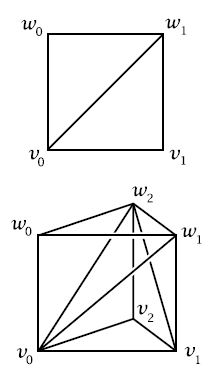
\includegraphics[width=4cm]{cilindrosimplice}
%\end{wrapfigure} 
%------------------------------------------
\def\windowpagestuff{\flushright 
   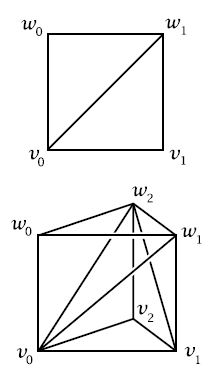
\includegraphics[width=2.8cm,height=4.5cm]{cilindrosimplice}}
   
  
   \begin{cutout}{1}{0.75\textwidth}{0pt}{6}
     \noindent
El primer paso será subdividir $\Delta^n\times I$ en simplices. Sea $\Delta^n\times\{0\}=[v_0,\dots, v_n]$ y $\Delta^n\times\{1\}=[w_0,\dots, w_n]$, donde $v_i$ tiene la misma imagen que $w_i$ mediante la proyección $\Delta^n\times I\to \Delta$. Para cada $0\leq i\leq n$ consideramos el $(n-1)$-símplice $[v_0,\dots, v_i, w_i,\dots, w_n]$. Este símplice se ha conseguido simplemente recorriendo $\Delta^n\times\{0\}$ hasta el vértice $v_i$ y después saltando a $w_i$ para recorrer el resto de $\Delta^n\times\{1\}$, para luego volver a $v_0$. La figura muestra los casos $n=1,2$.
\end{cutout}\
%INTENTAR CON CUTWIN \url{https://tex.stackexchange.com/questions/40806/how-to-wrap-text-around-a-figure-revised}
%\begin{figure}[h!]
%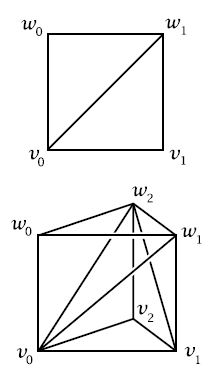
\includegraphics[scale=0.7]{cilindrosimplice}
%\end{figure}

Dada una homotopía $F:X\times I\to Y$ y un símplice singular $\sigma:\Delta^n\to X$, podemos formar la composición $F\circ(\sigma\times Id):\Delta^n\times I\to X\times I\to Y$. Usando esto podemos definir el \emph{operador prisa} $P:C_n(X)\to C_{n+1}(Y)$ como sigue
\[
P(\sigma)=\sum_i(-1)^iF\circ(\sigma\times I)|_{[v_0,\dots, v_i, w_i,\dots, w_n]}
\]
Vamos a demostrar que el operador prisma satisface la relación
\[
dP=g_*-f_*-Pd
\]
Para probarlo calculamos
\[
dP(\sigma)=\sum_{j≤i}
(−1)^i(−1)^jF\circ(σ \times Id)|_{ 
[v_0, \dots, \hat{v}_j , \dots ,v_i,w_i, \dots ,w_n]}
+\sum_{j≥i}
(−1)^i(−1)^{j+1}F\circ(σ\times Id)|_{
[v_0, \dots ,v_i,w_i, \dots ,\hat{w}_j , \dots ,w_n]}
\]
Los términos para $i=j$ se cancelan excepto para $F\circ(σ \times Id)|_{ 
[\hat{v}_0,w_0,\dots ,w_n]}$, que es $g\circ\sigma=g_*(\sigma)$; y $-F\circ(σ \times Id)|_{ 
[v_0,,\dots ,v_n,\hat{w}_n]}$, que es $-f\circ \sigma=-f_*(\sigma)$. Los términos para $i\neq j$ son exactamente $-Pd(\sigma)$. 

Así, si $\alpha\in Z_n(X)$, entonces $g_*(\alpha)-f_*(\alpha)=Pd(\alpha)+dP(\alpha)=dP(\alpha)$ por ser $d\alpha=0$. Entonces $g_*(\alpha)$ y $f_*(\alpha)$ determinan la misma clase de homología al ser su diferencia un borde. 
%Para el caso aumentado creo que P=0 (comprobar).
\end{dem}

En la prueba hemos usado la relación $dP-Pd=f_*-g_*$, que es la que define una \emph{homotopía de complejos de cadenas} entre $f_*$ y $g_*$ (se denota en ese caso $f_*\simeq g_*$). Una \emph{equivalencia de homotopía} enre complejos de cadenas $f:C_*\to D_*$ es un morfismo de complejos de cadenas tal que existe $g:D_*\to C_*$ de modo que $g\circ f\simeq Id_{C_*}$ y $f\circ g\simeq Id_{D_*}$.  Hemos probado además que una equivalencia de homotopía de complejos de cadenas induce isomorfismo en la homología. Para el caso de homología reducida también es válido este resultado definiendo $f_*:\Z\to\Z$ como 0 y $P:\Z\to C_0(Y)$ como la aplicación nula.

\begin{coro}
Si $f:X\to Y$ es equivalencia homotópica, entonces $f_*$ es isomorfismo.
\end{coro}

\section{Álgebra Homológica}

Asumimos conocidas las definiciones y propiedades básicas de las sucesiones exactas. 

\begin{lemma}[Splitting lemma]
Dada una sucesión exacta de módulos $0\to A\xrightarrow{f}B\xrightarrow{g}C\to 0$ son equivalentes:
\begin{enumerate}[a)]
\item Hay un morfismo $p:B\to A$ tal que $pf=Id:A\to A$.
\item Hay un morfismo $s:C\to B$ tal que $gs=Id:C\to C$. 
\item Existe un isomorfismo $B\cong A\oplus C$ compatible con la sucesión exacta corta, es decir, que hace conmutar el siguiente diagrama
\[
\begin{tikzcd}
A\arrow[r, rightarrowtail, "f"]\arrow[d, equals] & B\arrow[r, twoheadrightarrow, "g"]\arrow[d, "u"] & C\arrow[d, equals] \\
A\arrow[r, "i"] & A\oplus C\arrow[r, "\pi"]& C
\end{tikzcd}
\]
\end{enumerate}
\end{lemma}
\begin{proof}
Que c) implica a) y b) es trivial.

Para ver que a) implica c), sea $p:B\to A$ un homomorfismo que verifique $pf=Id$. En este caso, afirmamos que $B=f(A)\oplus\ker p$. Si $b\in B$, entonces $b=fp(b)+(m-fp(b))$. Es claro que $fp(b)\in f(A)$ y además $p(b-fp(b)=p(b)-pfp(b)=p(b)-p(b)=0$, luego $b-fp(b)\in\ker p$. Se tiene también que si $b\in f(A)\cap\ker p$, entonces $b=f(a)$ y $0=p(b)=pf(a)=a$, por lo que $b=0$, con lo que la afirmación es cierta. Una vez que tenemos $b=f(a)+b'$, definimos el homomorfismo $u(b)=a+g(b')$. Se tiene de hecho que $u(b)=a+g(b)$, pues si $b-b'=f(a)$ y por exactitud $g(b-b')=0$. Esta definición no es ambigua por ser $f$ inyectiva. Por la definición que se ha hecho, el diagrama es conmutativo y el lema de los 5 implica que $u$ es isomorfismo.

Por último veamos que b) implica c). Sea $s:C\to B$ tal que $gs=Id$. Afirmamos que $B=\ker g\oplus s(C)$. Sea $b\in B$, lo escribimos como $b=(b-sg(b))+sg(b)$. Es claro que $sg(b)\in s(C)$ y además $g(b-sg(b))=g(b)-gsg(b)=g(b)-g(b)=0$, por lo que $b-sg(b)\in\ker g$. Si $b\in\ker g\cap s(C)$, entonces $b=s(c)$ y $0=g(b)=gs(c)=c$, por lo que $b=0$, lo que prueba la afirmación. Ahora, como $\ker g=\Ima f$, podemos expresar $b=f(a)+s(c)$. Definimos entonces $u(b)=a+c$, lo cual tiene sentido porque tanto $f$ como $s$ son inyectivas y además $\Ima s\cap\Ima f=\Ima s\cap\ker g=0$. La definición que hemos hecho hace conmutar el diagrama y esto hace que $u$ sea isomorfismo por el lema de los cinco. 
\end{proof}

Cuando $C$ es un objeto proyectivo se verifica la escisión. En particular, cuando sea un objeto libre. Se recuerda que una sucesión de complejos  de cadenas $0\to A^*\to B^*\to C^*\to 0$ se dice exacta si lo es en cada nivel. Se advierte que el hecho de que se tenga escisión en cada nivel no implica que $B^*\cong A^*\oplus C^*$ pues los isomorfismos de cada nivel no tienen por qué ser compatibles con el operador borde. 

\begin{teorema}
Toda sucesión exacta corta de complejos de cadenas $0\to A\xrightarrow{f} B\xrightarrow{g} C\to 0$ induce una sucesión exacta larga
\[
\cdots \to H_n(A)\xrightarrow{f_*}H_n(B)\xrightarrow{g_*}H_n(C)\xrightarrow{\partial}H_{n-1}(A)\to\cdots
\] 
%\xrightarrow[g] pone la g debajo
\end{teorema}
La prueba sigue la clásica estrategia de \emph{diagram chasing} y se puede encontrar a partir de la página 116 de \emph{Algebraic Topology} de Allen Hatcher. 
\section{Homología relativa}

Dado un subespacio $A\subseteq X$, vamos a construir el complejo de cadenas relativo $C_*(X,A)$ asociado al par $(X,A)$, lo que nos dará la homología relativa $H_*(X,A)$. Esto se consigue definiendo $C_n(X,A)=C_n(X)/C_n(A)$. Este cociente tiene sentido porque $A\subseteq X$ y entonces el complejo está contenido mediante la aplicación inducido por la inclusión. Como $d$ lleva $C_n(A)$ en $C_{n-1}(A)$, podemos definir $d:C_n(X,A)\to C_{n-1}(X,A)$ como $d([x])=[d(x)]$. Así, la homología relativa es la homología del complejo de cadenas $H_n(X,A)=H_n(C_*(X,A))$. 

A partir de las sucesión exacta corta evidente $0\to C_*(A)\to C_*(X)\to C_*(X,A)\to 0$ surge la sucesión exacta larga de homología relativa
\[
\cdots \to H_n(A)\xrightarrow{f_*}H_n(X)\xrightarrow{g_*}H_n(X,A)\xrightarrow{\partial}H_{n-1}(A)\to\cdots
\]

También existe el análogo reducido de esta sucesión exacta larga para un par $(X,A)$ donde $A\neq\emptyset$, obtenida a partir de las sucesiones exactas cortas $0\to C_n(A)\to C_n(X)\to C_n(X,A)\to 0$ aumentadas en dimensión $-1$ por $0\to\Z\xrightarrow{Id}\Z\to 0\to 0$. En particular, esto significa que $\widetilde{H}_n(X,A)=H_n(X,A)$ para todo $n$ si $A\neq\emptyset$.

\begin{defi}
Una aplicación de pares $f:(X,A)\to (Y,B)$ es una aplicación $f:X\to Y$ tal que $f(A)\subseteq B$. 
\end{defi}

Una aplicación de pares induce una aplicación $f|_A:A\to B$, así que se puede definir un morfismo de complejos de cadenas inducido por $f$, $f_*:C_*(X,A)\to C_*(Y,B)$ como $[c]\mapsto [f_*(c)]$ que cumple las propiedades de funtorialiad. Por tanto da lugar también a un homomorfismo en homología $f_*:H_*(X,A)\to H_*(Y,B)$, que es natural con respecto a la sucesión exacta larga de homología relativa, es decir, conmuta el diagrama 
\[
\begin{tikzcd}
\cdots \to H_n(A)\arrow[r]\arrow[d, "f|_{A*}"] & H_n(X)\arrow[r]\arrow[d, "f_*"] & H_n(X,A)\arrow[d, "f_*"]\arrow[r] &H_{n-1}(A)\arrow[d]\to\cdots\\
\cdots \to H_n(B)\arrow[r] & H_n(Y)\arrow[r] & H_n(X,B)\arrow[r]& H_{n-1}(B)\to\cdots
\end{tikzcd}
\]

ya que la conmutatividad se tiene ya a nivel de complejos de cadenas, y la conmutatividad con $\partial$ se puede probar. 
 

\begin{teorema}[de excisión]\label{excision}
Sean subespacios $Z\subseteq A\subseteq X$ tal que la clausura de $Z$ está en el interior de $A$. Entonces la inclusión $i:(X-Z,A-Z)\hookrightarrow (X,A)$ induce isomorfismos $i_*:H_n(X-Z,A-Z)\to H_n(X,A)$ para todo $n$. Equivalentemente, para subespacios $A,B\subseteq X$ cuyos interiores cubren $X$, la inclusión $(B,A\cap B)\hookrightarrow (X,B)$ induce isomorfismos $H_n(B,A\cap B)\to H_n(X,B)$ para todo $n$. 
\end{teorema}

Para un espacio $X$, consideremos una familia de subconjuntos $\mathcal{U}=\{U_i\}_{i\in I}$ tales que $X=\cup_i int(U_i)$. Decimos que un símplice singular en $X$, $\sigma:\Delta^n\to X$ está \emph{subordinado} a $\mathcal{U}$ si existe $I\in I$ con $\delta(\Delta^n)\subseteq U_i$. Denotamos $C^{\mathcal{U}}_*$ al complejo de cadenas de símplices de $X$ subordinados a $\mathcal{U}$, que está contenido en $C_*(X)$.  El operador borde está bien definido, puesto que si $\sigma:\Delta^n\to X$ es tal que $\sigma(\Delta^n)\subseteq U_i$ y si $\Delta^n_i$ es la $i$-ésima cara de $\Delta^n$, entonces $d(\sigma)=\sum_{i=0}^n(-1)^i\sigma|_{\Delta^n_i}$. Como $\sigma(\Delta^n)\subseteq U_i$, también lo está la restricción a cada una de las caras.

\begin{teorema}[de las cadenas pequeñas]\label{peque}
La inclusión $C^{\UU}_*(X)\hookrightarrow C_*(X)$ es una equivalencia homotópica de complejos de cadenas. 
\end{teorema}

\begin{defi}
El \emph{baricentro} de un símplice $\sigma=[v_0,\dots, v_n]$ es $b(\sigma)=\sum_{i=0}^n\frac{1}{n+1}v_i\in \sigma$. La \emph{subdivisión baricéntrica} es el complejo simplicial formado por los baricentros de las caras de $\sigma$. La $k$-ésima subdivisión baricéntrica es la división baricéntrica de la $k-1$-ésima subvidisión baricéntrica.
\end{defi}

En general, si $\sigma$ es un símplice y dados $\sigma_0\leq\cdots\sigma_t\leq\sigma$, se tiene que $[b(\sigma_0),\dots, b(\sigma_t)]$ forma un símplice contenido en $\sigma$. 

Se define el \emph{diámetro} de $\sigma\subseteq \R^N$ como $dia(\sigma)=\max_{x,y\in\sigma} d(x,y)$. Denotamos $d(x,y)$ como $|x-y|$. Dados $x,y\in\sigma$, con $y=\sum_{i=0}^n t_iv_i$ y $\sum_{i=0}^nt_i=1$, 
\[
|x-y|=\left|\sum_{i=0}^nt_ix-\sum_{i=0}^nt_iv_i\right|=\left|\sum_{i=0}^nt_i(x-v_i)\right|\leq \sum_{i=0}^n t_i|x-v_i|\leq \sum_{i=0}^nt_i\max_{j=0,\dots, n}|x-v_j|=\max|x-v_j|\leq \max|v_k-v_j|
\]

\begin{lemma}
 Si $\tau$ es un símplice de la subdivisión baricéntrica de $\sigma$, $\dim(\sigma)=n$, 
\[
dia(\tau)\leq\frac{n}{n+1}dia(\sigma)
\]
\end{lemma}

La demostración se puede encontrar en los apuntes de Homología Simplicial o alternativamente en Hatcher página 120. 

\begin{coro}
Si $\tau$ es un símplice de la $k$-ésima subdivisión baricéntrica de $\sigma$, $\dim(\sigma)=n$, 
\[
dia(\tau)\leq \left(\frac{n}{n+1}\right)^k dia(\sigma)
\]
\end{coro}

\begin{coro}\label{r}
Sea $\sigma$ un $q$-símplice sobre $X$ y $\mathcal{P}$ un recubrimiento por abiertos de $X$. Entonces $\exists r>0$ tal que $S^r(\sigma)$ es combinación lineal de símplices subordinados a $\mathcal{P}$, esto es, si $\mathbb{P}=\{V_i\}_{i\in I}$, existe $i\in I$ con $\Ima\sigma\in V_i$. 
\end{coro}
\begin{dem}
$\sigma$ es una aplicación continua que parte de un espacio métrico compacto, luego $\{\sigma^{-1}(V_i)\}$ es recubrimiento de $\Delta^q$. Tomamos $\varepsilon>0$ el número de Lebesgue de $\Delta_q$ respecto de $\sigma^{-1}(\mathcal{P})$. Entones existe $r>0$ tal que el diámetro de $S^r(\Delta_q))$ es menor que $\varepsilon$, por lo que $S^r(\sigma)$ está subordinado a $\mathcal{P}$. 
\end{dem}

\begin{dem}[del teorema de Excisión]
No usamos la estrategia de Hatcher sino de Greenberg, usando que $C_*^{\UU}(X,A)\to C_*(X,A)$ induce isomorfismo en homología. Definimos un morfismo de complejos de cadenas $S:C_q(X)\to C_q(X)$ llamado \emph{subdivisión} y una homotopía de complejos de cadenas $T:C_*(X)\to C_{*+1}(X)$ entre la identidad y $S$, es decir $dT+Td=Id-S$, que funcionarán de forma natural (como functores). En particular, si $\sigma:\Delta^q\to X$, tenemos el diagrama conmutativo
\[
\begin{tikzcd}
C_q(\Delta^q)\arrow[r, "S_q"]\arrow[d, "\sigma_*"] & C_q(\Delta^q)\arrow[d, "\sigma_*"]\\
C_q(X)\arrow[r, "S_q"] & C_q(X)
\end{tikzcd}
\] 
Si consideramos la identidad $\delta:\Delta^q\to\Delta^q\in C_q(\Delta^q)$, $\sigma=\sigma_*(\delta)\in C_q(X)$, entonces $S_q(\sigma)=\sigma_*(S_q(\delta))$. 

Tendremos luego un cubo como el siguiente 
\[
\begin{tikzcd}
&
C_q(\Delta^q)
\ar{dl}[swap, sloped, near start]{\sigma_*}
\ar{rr}{S_q}
\ar[]{dd}[near start]{d}
& & C_q(\Delta^q)
\ar{dd}{d}
\ar{dl}[swap, sloped, near start]{\sigma_*}
\\
C_q(X)
\ar[crossing over]{rr}[near end]{S_q}
\ar{dd}[swap]{d}
& & C_{q}(X)
\ar[crossing over]{dd}[]{d}
\\
&
C_{q-1}(\Delta^q)
\ar[near start]{rr}{S_{q-1}}
\ar[sloped, swap]{dl}{\sigma_*}
& & C_{q-1}(\Delta^q)
\ar[sloped, swap]{dl}{\sigma_*}
\ar{dl}
\\
C_{q-1}(X)
\ar{rr}{S_{q-1}}
& & C_{q-1}(X)
\ar[crossing over, leftarrow, near start]{uu}{}
\end{tikzcd}
\]
en el que todas las caras salvo la frontal habrán sido probadas conmutativas, pero la conmutatividad de esta cara se deduce de la del resto.

Vamos a definir entonces $S$ y $T$ inductivamente. $S(\delta_0)=\delta_0=T(\delta_0)$. $S_q(\delta_q)=B_q(S_{q-1}d\delta_q)$, donde $B_q$ es el cono sobre la subdivisión baricéntrica de $d(\delta_q)$ (recordemos que $\Delta_q$ es el cono de $\Delta_{q-1}$, que podemos tomar con vértice extra un punto que tiene como proyección el baricentro de $\Delta_{q-1}$, y sobre una cadena no es más que una cadena de conos). Aunque no se vea muy intuitivo, a cada símplice le asocia la suma de los símplices de su subdivisión baricéntrica. $T_q(\delta_q)=B_q(\delta_q-S\delta_q-T_{q-1}(d\delta_q))$.

Veamos que $dS=Sd$. Si $q=0$, $dS=Sd=0$. Para $q>0$, 
\[
dS(\delta_q)=dS(\delta_q)=d(B_q(S_{q-1} d\delta_q))
\]
Ahora, $d(B\sigma)=\sigma-Bd\sigma$, pues $d([B,v_0,\dots, v_q])=[v_0,\dots, v_q]-Bd[v_0,\dots, v_q]$. Luego, aplicando hipótesis de inducción
\[
d(B_q(S_{q-1} d\delta_q))=S_{q-1}dS_q-B_q(dS_{q-1}d\delta_q)=S_{q-1}d\delta_q-B_qS_{q-1}ddS_q=S_{q-1}D(\delta_q)
\]

Ahora vemos que $dT+Td=Id-S$. 
\[
dT\delta_q=d(B_q(\delta_q-S\delta_q-TdS_q)=(\delta_q-S\delta_q+TdS_q)-B_q(d\delta_q-dS\delta_q-dTd\delta_q)=
\]
\[
(\delta_q-S\delta_q-Td\delta_q)-B_q(d\delta_q-Sd\delta_q-(d\delta_q-Sd\delta_q-Td(d\delta_q)))=
\]
\[
\delta_q-S\delta_q+Td\delta_q
\]

Tenemos ya entonces que $S_*=Id_*:H_q(X)\to H_q(X)$. Probamos ahora el siguiente resultado
\begin{lemma}
Sea $X$ un espacio topológico y $\mathcal{P}$ un recubrimiento por abiertos de $X$. Entonces, todo ciclo de $H_q(X,A)$ puede ser representado por un ciclo subordinado a $\mathcal{P}$.
\end{lemma}
\begin{proof}
Dado $[z]\in H_q(X,A)$, $z$ es un ciclo relativo, luego $d(z)$ es un borde relativo, así que es una cadena en $A$. Además $z-S(z)=dT(z)+Td(z)$. Se tiene que $Td(z)$ tiene imagen en $A$, luego $z\equiv S(z)+dT(z)\mod A$. Así que $[z]=[S(z)]\in H_q(X,A)$. Inductivamente obtenemos $[z]=S^r(z)]\in H_q(X,A)$, luego basta tomar $r>0$ como en el corolario \ref{r}. 
\end{proof}

Finalmente podemos probar que $i_*:H_q(X-Z,A-Z)\to H_q(X,A)$ es isomorfismo. Primero vemos que es sobreyectiva. Sea $[z]\in H_q(X,A)$, $z=\sum\lambda_i\sigma_i$ subordinado a $\{int A, X-\overline{Z}\}$, esto es, cualquier $\sigma_i$ cuya imagen no caiga en $X-Z\supseteq X-\overline{Z}$, verifica que su imagen cae en $int(A)\subseteq A$, luego los podemos eliminar. Podemos suponer entonces que $X$ cae $X-Z$, luego $[z]$ define una clase  en $H_q(X-Z,A-Z)$. 

Ahora probamos que $i_*$ es inyectiva. Si $[z]\in H_q(X-Z,A-Z)$ es tal que $i_*[z]=0\in H_q(X,A)$, esto quiere decir que $z=z'+dw$ para $w\in C_{q-1}(X,A)$ y $z'\in C_q(A)$. Elegimos $r>0$ de modo que $S^r(z)$ esté subordinado a $\{intA, X-\overline{Z}\}$. Así $S^r(z)=S^r(z')+d(S^r(w))$. Por un lado, $S^r(w)=w_q+w_2$, donde $w_1$ tiene símplices singulares en $X-\overline{Z}$ y $w_2$ en $int(A)$. De modo que $S^r(z)-dw_1=S^r(z')+dw_2$, donde el término de la izquierda está en $X-Z$ y el de la derecha en $A$, luego tienen que caer en $A-Z$. Así que $S^r(z)\simeq 0$ en $X-Z\mod A-Z$, es decir $[z]=[S^r(z)]=0\in H_q(X-Z,A-Z)$.  
\end{dem}


\begin{prop}
Si $f:(X,A)\to (Y,B)$ es una aplicación de pares tal que tanto $f:X\to Y$ como $f|_A:A\to B$ son equivalencias de homotopía, entonces $f$ como aplicación depares induce isomorfismos en homología relativa $f_*:H_n(X,A)\to H_n(Y,B)$ para todo $n\in\Z$.
\end{prop}
\begin{dem}
Es trivial a partir de las sucesiones largas de homología relativa respectiva, que equivalencias de homotopía inducen isomorfismos y el lema de los cinco.
\end{dem}

\begin{defi}
Un \emph{buen par} $(X,A)$ es un par tal que $A\subseteq X$ es cerrado y existe un abierto $U$ con $A\subseteq U\subseteq X$ tal que $A$ es retracto de deformación fuerte de $U$.
\end{defi}


\begin{prop}
Sea $X$ un espacio y $x_0\in X$. Entonces $\widetilde{H}_n(X)\cong\widetilde{H}_n(X,x_0)=H_n(X,x_0)$.
\end{prop}
\begin{dem}
Como $\widetilde{H}_*(x_0)=0$, al sustituir en la sucesión exacta larga de homología relativa tenemos los isomorfismos buscados.
\end{dem}

\begin{prop}\label{2.22}
Si $(X,A)$ es un buen par, entonces $(X,A)\to (X/A,A/A)$ induce isomorfismos $H_n(X,A)\cong H_n(X/A,A/A)\cong\widetilde{H}_n(X/A)$ para todo $n\in\Z$. 
\end{prop}
\begin{dem}
Consideremos el diagrama conmutativo siguiente.
\[
\begin{tikzcd}
H_n(X,A)\arrow[d,"p_*"]\arrow[r,"i_*"] & H_n(X,U)\arrow[d]&H_n(X-A,U-A)\arrow[l]\arrow[d]\\
H_n(X/A,A/A)\arrow[r, "i_*"]& H_n(X/A, U/A) &\arrow[l]H_n((X/A)-[A], (U/A)-[A])
\end{tikzcd}
\]
Se tiene que $i_*:H_n(X,A)\to H_n(X,U) $ es isomorfismo porque está inducido por la inclusión y $A$ es retracto de deformación fuerte de $U$. Esta retracción pasa al cociente y $[A]$ es retracto fuerte de $U/A$. Las flechas horizontales de la derecha son isomorfismos por excisión. Como la aplicación cociente es homeomorfismo fuera de $A$, la flecha vertical de la derecha es isomorfismo, al estar inducida por un homeomorfismo de pares. Por conmutatividad también es isomorfismo la flecha central. De nuevo por conmutatividad es isomorfismo $p_*$, que era lo que queríamos probar. 
\end{dem}

\begin{teorema}
Si $(X,A)$ es un buen par, entonces tenemos una sucesión exacta larga
\[
\cdots\to \widetilde{H}_n(A)\xrightarrow{i_*}\widetilde{H}_n(X)\xrightarrow{p_*}\widetilde{H}_n(X/A)\to\widetilde{H}_{n-1}(A)\to\cdots
\]
donde $i:A\to X$ es la inclusión y $p:X\to X/A$ es la proyección.
\end{teorema}

\begin{ej}
$$\widetilde{H}_*(S^n)=\begin{cases}
\Z & *=n\\
0 & *\neq n
\end{cases}$$

Lo hacemos por inducción. Para $n=0$, $S^0$ es un espacio discreto formado por dos puntos, de donde se deduce el resultado. Para $n>0$ usamos que $S^n=D^n/S^{n-1}$ y usamos la sucesión exacta larga de homología reducida con el cociente. Como $D^n$ es contráctil, tenemos isomorfismos $\widetilde{H}_k(S^n)\cong\widetilde{H}_{k-1}(S^{n-1})$ de donde se deduce el resultado. 
\end{ej}

\begin{teorema}[del punto fijo de Brouwer]
Toda apliación continua $f:D^n\to D^n$ tiene al menos un punto fijo.
\end{teorema}
\begin{dem}
Si $f$ no tiene puntos fijos, $x-f(x)\neq 0$, luego $g(x)$ definida como el punto de corte de la semirrecta que va de $f(x)$ a $x$ con $S^{n-1}$  es una aplicación continua $g:D^n\to S^{n-1}$ que restringe a la identidad en $S^{n-1}$. Tenemos entonces la descomposición de la identidad
\[
S^{n-1}\hookrightarrow D^n\xrightarrow{g}S^{n-1}
\] 
Esto induce por functorialidad una descomposición de la identidad
\[
\Z=H_{n-1}(S^{n-1})\xrightarrow{i_*}H_{n-1}(D^n)=0\xrightarrow{g_*}H_{n-1}(S^{n-1})=\Z
\]
Esto implicaría que $Id:\Z\to\Z$ es la aplicación nula, contradicción.

\end{dem}

\begin{ej}
Consideramos el par $(D^n,S^{n-1})$. La homología de este par es $$H_*(D^n,S^{n-1})=\begin{cases}
\Z & *=n\\
0 & *\neq n
\end{cases}$$

Esto se puede probar a partir de la sucesión exacta larga de homología reducida usando que para $k>0$, la reducida es igual que la no reducida, pero en este ejemplo estamos interesados en encontrar generadores. Tenemos el homeomorfismo $D^n\cong\Delta^n$ y $S^{n-1}\cong\partial\Delta^n$. Así que $(D^n,S^{n-1})\cong (\Delta^n, \partial\Delta^n)$. Vamos a buscar un generador de la homología no trivial. $H_n(\Delta^n,\partial\Delta^n)\cong\Z$. La identidad $Id:\Delta^n\to\Delta^n$ es un ciclo relativo porque el borde es una suma de símplices singulares que caen en $\partial\Delta^n$. Vamos a ver que $[Id]$ es un generador. Lo hacemos por inducción. En $n=0$, como $\partial\Delta^0=\emptyset$, $H_0(\Delta^0,\emptyset)=H_0(*)\cong\Z$ generado por la única aplicación posible, que es la identidad. Para $n>0$, suponiendo que es cierto para $n-1$, tenemos un isomorfismo $H_n(\Delta^n,\partial\Delta^n)\cong \widetilde{H}_{n-1}(\partial\Delta^n)$ en la sucesión exacta larga del par, dado por la aplicación que conecta las dimensiones. A su vez, $\widetilde{H}_{n-1}(\partial\Delta^n)\cong \widetilde{H}_{n-1}(\partial\Delta^n,v_n)$ para $v_n$ un vértice del símplice. Este isomorfismo proviene de la sucesión exacta larga del par $(\partial\Delta^n,v_n)$ usando que la homología reducida del vértice es trivial. Además, la homología reducida es igual a la no reducida en pares donde el segundo elemento no sea vacío. Consideramos la cara $\Delta^{n-1}=[v_0,\dots, v_{n-1}]$ y denotamos $\Lambda=\partial\Delta^n-int(\Delta^{n-1})$, que es contráctil por ser el cono el borde de $\Delta^{n-1}$. Así que tenemos un isomorfismo $H_{n-1}(\partial\Delta^n,v_n)\cong H_n(\partial\Delta^n,\Lambda)$. Ahora consideramos $H_{n-1}(\Delta^{n-1},\partial\Delta^{n-1})\to H_{n-1}(\partial\Delta^n,\Lambda)$ inducido por la inclusión. Vamos a ver que es un isomorfismo. Es claro que estos pares son buenos. Por lo que $H_{n-1}(\Delta^{n-1},\partial\Delta^{n-1})\cong \widetilde{H}_{n-1}(\Delta^{n-1}/\partial\Delta^{n-1})$ y $H_{n-1}(\partial\Delta^n,\Lambda)\cong\widetilde{H}_{n-1}(\partial\Delta^n/\Lambda)$. Como $\widetilde{H}_{n-1}(\Delta^{n-1}/\partial\Delta^{n-1})\cong  \widetilde{H}_{n-1}(\partial\Delta^n/\Lambda)$ por ser los espacios homeomorfos, la naturalidad nos da el isomorfismo que buscábamos (ver diagrama).
\[
\begin{tikzcd}
H_{n-1}(\Delta^{n-1},\partial\Delta^{n-1})\arrow[r, "i_*", "\cong"']\arrow[d, "\cong"] & H_{n-1}(\partial\Delta^n,\Lambda)\arrow[d]\\
\widetilde{H}_{n-1}(\Delta^{n-1}/\partial\Delta^{n-1})\arrow[r, "\cong"] & \widetilde{H}_{n-1}(\partial\Delta^n/\Lambda)
\end{tikzcd}
\] 

Nuestra hipótesis de inducción nos da que $[Id_{\Delta^{n-1}}]$ genera $H_{n-1}(\Delta^{n-1},\partial\Delta^{n-1})$. Si consideramos $Id_{\Delta^n}\in C_n(\Delta^n)$, $d(Id_{\Delta^n})\in C_{n-1}(\Delta^n)$ y además $d(Id_{\Delta^n})\in C_{n-1}(\partial\Delta^n)$. Ahora, salvo signo, $[Id_{\Delta^{n-1}}]\mapsto [d(Id_{\Delta^n})]\in H_{n-1}(\partial\Delta^n,\Lambda)$, que es también ciclo en $H_{n-1}(\partial\Delta^n,v_n)$. Con el isomorfismo que teníamos previamente, tenemos también que es generador de $\widetilde{H}_{n-1}(\partial\Delta^n)$, y atendiendo a la definición de la aplicación que conecta dimensiones, $[Id_{\Delta^n}]\mapsto [d(Id_{\Delta^n})]$, con lo que hemos encontrado el generador. 


Ahora bien, como $H_n(D^n,S^{n-1})\cong \widetilde{H}_n(S^n)$ es isomorfismo, siendo $(D^n,S^{n-1})$ un buen par tal que $D^n\xrightarrow{p}D^n/S^{n-1}\cong S^n$, tenemos $[\Delta^n\xrightarrow{Id}\Delta^n\cong D^n]\mapsto [\Delta^n\xrightarrow{Id}\Delta^n\xrightarrow{p}S^n]$. 

Otra forma de hacerlo es la siguiente: podemos expresar $S^n$ como $\Delta^n_1\bigcup_{\partial\Delta^n}\Delta^n_2$, de modo que ambos símplices están incluidos en $S^n$ por $i_1$ e $i_2$. Tendríamos $d(i_1)=d(i_2)$, por lo que $[i_1-i_2]$ es un generador, que se mapea al generador $[i_1-i_2]=[i_1]\in \widetilde{H}_n(S^n,\Delta^n_2)$, que a su vez es la imagen de $[Id_{\Delta^n}]$ mediante el isomorfismo que viene de $\widetilde{H}_n(\Delta^n_1,\partial\Delta^n)$ (es isomorfismo porque está inducido por un homeomorfismo). Más detalles en el ejemplo 2.23 de Hatcher.
\end{ej}

\begin{coro}
Para un wedge $\bigvee_{\alpha} X_{\alpha}$, las inclusiones $X_{\alpha}\hookrightarrow\bigvee_{\alpha} X_{\alpha}$ induce isomorfismos $\oplus_{\alpha}i_{\alpha *}:\oplus_{\alpha} \widetilde{H}_n(X_{\alpha})\to  \widetilde{H}_n(\bigvee_{\alpha} X_{\alpha})$, suponiendo que el wedge está formado en puntos base $x_{\alpha}\in X_{\alpha}$ tales que $(X_{\alpha},x_{\alpha})$ son buenos pares.
\end{coro}
\begin{dem}
Como la homología reducida es la misma que la homología relativa a un punto, se sigue de la proposición \ref{2.22}, tomando $(X,A)=(\sqcup_{\alpha} X_{\alpha}, \sqcup_{\alpha}\{x_{\alpha}\})$.
\end{dem}

\begin{teorema}
Si dos subconjuntos no vacíos $U\subseteq\R^m$ y $V\subseteq\R^m$ son homeomorfos, entonces $m=n$. 
\end{teorema}
\begin{dem}
Sea $x\in U$, por excisión $H_q(U,U-\{x\})\cong H_q(\R^m, \R^m-\{x\})$. De la sucesión exacta larga reducida del par $(\R^m, \R^m-\{x\})$ obtenemos $H_q(\R^m, \R^m-\{x\})\cong \widetilde{H}_{q-1}(\R^m-\{x\})$. Como $\R^m-\{x\}$ retrae con deformación fuerte sobre $S^{m-1}$, $\widetilde{H}_{q-1}(\R^m-\{x\})=\widetilde{H}_{q-1}(S^{m-1})=\delta_{qm}\Z$. Haciendo lo mismo con $\R^n$, como dos espacios homeomorfos tienen la misma homología, deducimos que $n=m$. 
\end{dem}


Generalizando la estrategia de la demostración anterior, definimos la \emph{homología local} de $X$ en $x$ como $H_*(X, X-\{x\})$. La homología local es un invariante topológico. En variedades topológicas, la homología local distingue puntos del borde.


Generalizando las sucesiones exacta larga de pares, podemos hacerla para una tripleta $(X,A,B)$. Esta tripleta da lugar a 3 parejas $(X,A)$, $(X,B)$, $(A,B)$ de donde obtenemos el diagrama de sucesiones exactas siguientes
\[
\begin{tikzcd}
C_*(A,B)\arrow[r, rightarrowtail] & C_*(X,B)\arrow[dr, twoheadrightarrow]&\\
C_*(A)\arrow[r, rightarrowtail] \arrow[u,twoheadrightarrow] & C_*(X)\arrow[r, twoheadrightarrow] \arrow[u,twoheadrightarrow]& C_*(X,A)\\
C_*(B)\arrow[u, rightarrowtail]\arrow[ur, rightarrowtail]& & 
\end{tikzcd}
\]
La sucesión exacta superior nos da la sucesión exacta larga
\[
\cdots\to H_n(A,B)\to H_n(X,B)\to H_n(X,A)\to H_{n-1}(A,B)\to\cdots
\]


\section{Grado}
Dada una aplicación continua $f:S^n\to S^n$, se induce un homomofismo $f_*:H_n(S^n)\to H_n(S^n)$, que no es más que un homomorfismo $\Z\to\Z$, que viene dado por $f_*(1)$, a lo cual llamamos \emph{grado} de $f$, denotado $\deg(f)$. 
\begin{propi}
Algunas propiedades sencillas son
\begin{enumerate}
\item $\deg(Id_{S^n})=1$.
\item $\deg(g\circ f)=\deg(f)\deg(g)$.
\item Si $f$ no es sobreyectiva, $\deg(f)=0$. 
\item Si $f\simeq g$, $\deg(f)=\deg(g)$. El recíproco es cierto, y es un resultado fundamental de Hopf en 1925. Se prueba usando que $\pi_n(S^n)=\Z$ y el grado nos da una aplicación $\pi_n(S^n)=\Z\to\Z$ sobreyectiva, luego tenemos una sucesióne exacta $0\to\ker(\deg)\to \Z\to\Z\to 0$. Como el rango del objeto central es la suma de los de los lados en este caso, $\ker(\deg)=0$. 
\item Si $f$ es una reflexión, entonces $\deg(f)=-1$, ya que intercambia los generadores norte y sur de $S^n$. 
\item Si $f=-Id_{S^n}$ (antipodal), $\deg(f)=(-1)^{n+1}$ por ser composición de $n+1$ reflexiones.
\item Si $f$ no tiene puntos fijos, $\deg(f)=(-1)^{n+1}$, puesto que existe una una homotopía entre $f$ y la antipodal dada por el segmento $(1-t)f(x)-tx$ (que no se anula) normalizado. 
\end{enumerate}
\end{propi}


\begin{prop}\label{suspension}
$\deg(Sf)=\deg(f)$, donde $Sf:S^{n+1}\to S^{n+1}$ es la suspención de la aplicación $f:S^n\to S^n$. 
\end{prop}
\begin{dem}
Consideramos el cono $CS^n$. La aplicación $(CS^n,S^n)\to (CS^n,S^n)$ inducida por $f$ es una aplicación de parejas. Entonces tenemos el diagrama siguiente, donde los 0 se obtienen de la sucesión exacta larga de homología relativa al ser $CS^n$ contráctil
\[
\begin{tikzcd}
           & \widetilde{H}_n(SS^n)\arrow[d, "\cong"]& &\\
0\arrow[r] & H_{n+1}(CS^n, S^n)\arrow[r, "\cong"]\arrow[d, "f_*"] &\widetilde{H}_n(S^n)\arrow[r] & 0\\
           & H_{n+1}(CS^n, S^n)\arrow[r, "\cong"]\arrow[d, "\cong"] &\widetilde{H}_n(S^n)& \\
           & \widetilde{H}_n(CS^n/S^n)\arrow[d,"\cong"] & & \\
           & \widetilde{H}_n(SS^n)& &
\end{tikzcd}
\]
La aplicación resultante $H_n(SS^n)\to H_n(SS^n)$ tiene el mismo grado que $f$ por conmutatividad, ya que los isomorfismos aunque envíen el 1 al $-1$ como se hacen dos veces se compensan. 
\end{dem}

Entendemos acción de un grupo $G$ sobre un espacio $X$ como una aplicación $G\to Homeo(X)$. 

\begin{prop}
Si $n$ es par, el único grupo que actúa libremente sobre $S^n$ es $\Z_2$. 
\end{prop}
\begin{dem}
Como un homeomorfismo tiene grado $\pm 1$, una acción de un grupo $G$ sobre la esfera define un homomorfismo $d:G\to\{\pm 1\}\cong\Z_2$. Como la acción es libre, $d$ envía cualquier elemento no trivial a $(-1)^{n+1}=-1$, puesto que el homeomorfismo inducido por un elemento será totalmente distinto de la identidad y por tanto será homotópico a la antipodal. Esto significa que $\ker(d)=1$, luego $G$ se inyecta en $\Z_2$. 
\end{dem}

Vamos a describir ahora una técnica que es útil para calcular el grado de un aplicación en la mayoría de casos. Sea $f:S^n\to S^n$ tal que existe $y\in S^n$ de modo $f^{-1}(y)=\{x_1,\dots, x_k\}$. Sean $U_i$ entornos disjuntos de $x_i$ tales que $y\in V=f(U_i)$. Para cada $i$, tenemos el siguiente diagrama. 
\[
\begin{tikzcd}
& H_n(U_i, U_i-x_i)\arrow[dl, "\cong"']\arrow[r, "f_*"]\arrow[d, "k_i"] & H_n(V, V-y)\arrow[d, "\cong"]\\
H_n(S^n, S^n-x_i) & H_n(S^n, S^n-f^{-1}(y))\arrow[l, "p_i"]\arrow[r, "f_*"] & H_n(S^n, S^n-y) \\
& H_n(S^n)\arrow[ul, "\cong"]\arrow[u, "j"']\arrow[r, "f_*"] & H_n(S^n)\arrow[u, "\cong"']
\end{tikzcd}
\]
Las aplicaciones $p_i$ y $k_i$ están inducidas por inclusiones. Los isomorfismos de abajo provienen de la sucesión exacta larga del par y los de arriba de la excisión. El de abajo a la izquierda es de nuevo por la pareja y el de encima por excisión también. Llamamos \emph{grado local} de $f$ en $x_i$ a $\deg(f|_{U_i})=\deg(f)|_{x_i}$. Si $f$ es homeomorfismo de $U_i$ en $V$, entonces $\deg(f)|_{x_i}=\pm 1$. En particular, si $f$ es homeomorfismo global, $y$ puede ser cualquier punto, que tendrá un solo punto preimagen $x_i$, con lo que $\deg(f)|_{x_i}=\deg(f)=\pm 1$.

\begin{prop}
$\deg(f)=\sum_i \deg(f)|_{x_i}$. 
\end{prop}
\begin{dem}
Como los $U_i$ son disjuntos, por escisión tenemos que $H_n(S^n, S^n-f^{-1}(y))=\oplus_i H_n(U_i, U_i-x_i)\cong\oplus_i\Z$, con $k_i(1)=(0,\dots,0, 1,0,\dots, 0)$ y $p_i$ es la $i$-ésima proyección. Entonces $p_i\circ k_i$ identidad. La conmutatividad del triángulo inferior da que $p_i\circ j(1)=1$, luego $j(1)=(1,\dots, 1)=\sum_ik_i(1)$. La conmutatividad del cuadrado superior dice que la $f_*$ del medio lleva $k_i(1)$ en $\deg(f)|_{x_i}$ (en la excisión el 1 va en el 1). Por lo tanto, $j(1)=\sum_ik_i(1)$ es enviado a $\sum_i \deg(f)|_{x_i}$. La conmutatividad del cuadrado inferior da la fórmula $\deg(f)=\sum_i \deg(f)|_{x_i}$.
\end{dem}

Vamos a ver ejemplos de cómo construir aplicaciones de grado arbitrario.

\begin{ej}
Sea $n>0$. Queremos construir una aplicación $f:S^n\to S^n$ de grado $k\in\Z$. Consideramos $q:S^n\to \bigvee_k S^n$ la aplicación cociente que surge al colapsar el complementario de $k$ discos disjuntos $B_i$ sobre $S^n$ sobre un punto. Y sea $p:\bigvee_k S^n\to S^n$ la aplicación consistente en identificar todas las esferas en una sola. Así que definimo $s=pq$. Para casi todos los puntos $y\in S^n$ (los que no son la imagen del punto común), $f^{-1}(y)$ consiste en $k$ puntos $x_i$, uno en cada $B_i$. El grado local de $f$ en $x_i$ es $\pm 1$ porque $f$ es homeomorfismo en un entorno de $x_i$. Componiendo $p$ con reflexiones en cada sumando de $\bigvee_k S^n$ si es necesario, podemos hacer que el grado local sea 1 (o $-1$), lo que el grado total de $f$ es la suma de los grados locales, que será $k$ (o $-k$). También podemos hacer que sea de grado $-k$ simplemente componiendo $f$ de grado positivo con una reflexión. Por la proposición \ref{suspension} podemos generar aplicaciones de grado arbitrario en esferas de dimensión mayor. 
\end{ej}

\begin{ej}
La aplicación $f:S^1\to S^1; z\mapsto z^k$ tiene grado $k>0$. Sea $x=1$, $f^{-1}(x)$ son las raíces $k$-ésimas de la unidad. Entonces $\deg(f)=\sum_{i^1}^k\deg(f)|_{y_i}$. En un entorno de $y_i$, $f$ es un homeomorfismo (simplemente hace más grande el intervalo y lo centra en $x$). Hay un homeomorfismo claro que hace exactamente lo mismo con este intervalo, consistente en un giro y una expansión en una mitad (con contracción en la otra). Esta aplicación es composición de dos aplicaciones homotópicas a la identidad, por lo que tienen grado 1. Así que el grado total es la suma de los grados de estas aplicaciones, es decir, $k$. El caso de $z^{-k}$, tenemos $z^{-k}=z^kz^{-1}$, y como $k^{-1}$ es el conjugado, se corresponde con una reflexión, luego tiene grado $-k$. Para $k=0$ es trivial porque es una aplicación constante.  
\end{ej}

\section{Homología celular}
\begin{defi}
Un $CW$-complejo es un espacio topológico $X$ equipado con una filtración $X^0\subset X^1\subset\cdots \subset X^n\subset\cdots\subset X$ tal que:
\begin{enumerate}
\item $X^0$ es un conjunto discreto de puntos. 
\item $X^{n+1}$ se construye a partir de $X^n$ ($n$-esqueleto) del siguiente como el pushout siguiente
\[
\begin{tikzcd}
\coprod_{\alpha}S^n_{\alpha}\arrow[r, hookrightarrow]\arrow[d, "\phi=(\phi_{\alpha})"] & \coprod_{\alpha}D^{n+1}_{\alpha}\arrow[d, "\overline{\phi}"]\\
X^n\arrow[r, hookrightarrow] & X^{n+1}
\end{tikzcd}
\]
Aquí $\phi_\alpha=\phi|_{S^n_{\alpha}}$. Tenemos que $\overline{\phi}$ es homeomorfismo sobre el interior de $D_{\alpha}^{n+1}$. Su imagen se denota $e^n_{\alpha}$ y se denomina \emph{celda abierta}. Se llaman \emph{celdas cerradas} son las clausuras $\overline{e}^n_{\alpha}\subseteq X$.  Los puntos son celdas abiertas y cerradas. 
\item $X=\bigcup_{n\geq 0} X^n$ con la topología débil, es decir, un subconjunto es cerrado si y solo si su intersección con todos los esqueletos es cerrado. 
\end{enumerate}
\end{defi}

Llamamos pushout al (único por propiedad universal) espacio que hace que este diagrama conmute
\[
\begin{tikzcd}
Y\arrow[r, hookrightarrow, "\iota"]\arrow[d, "f"] & Z\arrow[d, "\overline{f}"]\\
X\arrow[r, hookrightarrow, "\overline{\iota}"] & X\cup_f Z
\end{tikzcd}
\]
donde $X\cup_f Z=X\coprod Z/y\sim f(y)$, Obsérvese que realmente la aplicación $\overline{\iota}$ es una inclusión en el sentido de que no se están identificando puntos de $x$. Además $\overline{f}$ es homeomorfismo sobre el complementario de la imagen de $Y$. A $f$ se la llama aplicación de pegamiento y a $\overline{f}$ aplicación característica. 

Si $X=X^n$ y $X^n\neq X^{n-1}$, entonces $\dim X=n$. Dado un CW-complejo $X$, un \emph{subcomplejo} $Y\subseteq X$ es un CW-complejo $Y$ formado por la unión de celdas de $X$. En particular $Y^n\subseteq X^n$ y los esqueletos de $X$ son subcomplejos. El cociente de $X$ por $Y$ es un CW-complejo formado por las celdas de $X$ que no están en $Y$ y una 0-celda que representa a $Y$.

\begin{ej}
$S^n$ con una 0-celda y una $n$-celda. Otra forma es $S^n$ construido inductivamente como $S^{n-1}$ en el ecuador y dos $n$-celdas en los hemisferios, partiendo de $S^0$ como dos puntos (0-celdas). Esto es
\[
\begin{tikzcd}
S^{n-1}\coprod S^{n-1}\arrow[r, hookrightarrow]\arrow[d, "Id\coprod Id"] & D^n\coprod D^n\arrow[d]\\
S^{n-1}\arrow[r, hookrightarrow] & S^n
\end{tikzcd}
\]  
Se puede de hecho construir $S^{\infty}$ si no nos detenemos en ningún $n$. 
\end{ej}

\begin{ej}
El toro de puede conseguir con una 0-celda, dos 1-celdas y una 2-celda. Las dos 1-celdas provienen de las circunferencias generatrices, que intersecan en la 0-celda. El resto es una 2-celda.
\end{ej}

\begin{ej}[espacio proyectivo]
$\R P^n=B^n/(y\sim -y)$ para $y\in S^{n-1}$, que se puede ver como $\R P^{n-1}\cup_{\varphi} B^n$, es decir el espacio proyectivo de dimensión $n-1$ al que le pegamos una bola de dimensión $n$ mediante el pushout
\[
\begin{tikzcd}
B^n\arrow[r] & \R P^n\\
S^{n-1}\arrow[u, hookrightarrow]\arrow[r, "q"] & \R P^{n-1}=S^{n-1}/\sim\arrow[u]
\end{tikzcd}
\]
Así, $\R P^n=e^0\cup e^1\cup e^2\cup\cdots\cup e^n$. 

En el caso complejo hacemos la construcción análoga, en este caso $\C P^n=S^{2n+1}/(z\sim\lambda z)$ con $\lambda\in\C$ tal que $|\lambda|=1$. En el ejemplo 0.6 se puede ver que $\C P^n=\C P^{n-1}\cup B^{2n}$. Para ello, consideramos el conjunto de tuplas $(z_1,\dots, z_{n+1})$ con $z_{n+1}\in (0,+\infty)$. Todo elemento de $\C P^n$ tiene un representante en este conjunto multiplicando por $\overline{z}_{n+1}/|z_{n+1}|$. Este conjunto es a su vez el grafo de $w=(z_1,\dots, z_n)\mapsto \sqrt{1-|w|^2}$ (es obvio que $|w|\leq 1$). Por topología general, el grafo de cualquier aplicación continua $f:X\to Y$ es homeomorfo a $Y$ usando la proyección y la propia función. De aquí obtenemos que el grafo descrito es homeomorfo a $B^{2n}\supset S^{2n-1}$, conteniéndola como borde, exactamente para $|w|=1$. Aquí $B^{2n}$ se identifica con el hemisferio norte de $S^{2n}$. 

\end{ej}


\begin{ej}[cociente]
Sea $S^{n-1}=\{e^0, e^{n-1}\}\hookrightarrow D^n=\{e^0, e^{n-1}, e^n\}$. Entonces $D^n/S^{n-1}=\{e^0, e^n\}=S^n$. 
\end{ej}

\begin{observacion}
Si $K\subseteq X$ es un subcomplejo compacto, entonces $K$ toca a un número finito de células y por tanto está contenido en un subcomplejo de dimensión finita. En particular, esta propiedad se cumple para cada célula.
\end{observacion}

\begin{prop}
Dados $X,Y$ CW-complejos, el producto $X\times Y$ es un CW-complejo. Si las células de $X$ e $Y$ son respectivamente $\{e_\alpha^n\}$ y $\{e_{\beta}^m\}$, las del producto son $\{e_{\alpha,\beta}^{n+m}\}=\{e_\alpha^n\times e_\beta^m\}$.
\end{prop}

Obsérvese que $X\times Y$ en general no tiene la topología producto. Sí son la misma si $X$ o $Y$ son localmente compactos, que como CW-complejos se traduce en que alguno sea localmente finito. En general, $X\times Y$ como CW-complejo tiene la misma topología que $X\times Y$ con la topología generada por compactos, es decir, que un conjunto $A$ es cerrado si y solo si $A\cap K$ es compacto para cualquier $K$ compacto. 

\begin{ej}
El toro se puede obtener como $S^1\times S^1=\{e_{\alpha}^0,e_{\alpha}^1\}\times \{e_\beta^0,e_\beta^1\}$. En dimensión 0 hay una 0-célula que surge del producto de las dos 0-células; en dimensión 1 hay dos células y en dimensión 2 hay una. 
\end{ej}

Como consecuencia de que el producto y el cociente sea CW-complejo, la suspensión también lo es. Lo mismo pasa con el wedge product.

\begin{ej}[Join]
Dados $X,Y$ CW-complejos, su join se define como $X*Y=\{tx+(1-t)y\mid  x\in X,y\in Y, 0\leq t\leq 1\}/\sim =X\times Y\times I/\sim$, donde $X\times Y\times\{0\}\sim X$ y $X\times Y\times \{1\}\sim Y$. 
\end{ej}

\begin{ej}[smash product]
Se define el producto smash de $X$ e $Y$ como $X\land Y=X\times Y/X\lor Y$. Esto tiene sentido porque $X\times \{y_0\}\cup\{x_0\}\times Y\subseteq X\times Y$ y además la inversección de estos conjuntos es justamente $\{(x_0, y_0)\}$. Como ejemplo, tenemos que $S^n\land S^m=S^{n+m}$. Esto se ve claro en el caso $S^1\land S^1$ viendo $S^1\times S^1$ como el diagrama poligonal habitual del toro y colapsando el borde. 
\end{ej}



\begin{prop}
Si $X$ es un CW-complejo:
\begin{enumerate}
\item $\phi_{\alpha}:D_{\alpha}^n\to X$ se restringe a un homeomorfismo sobre $e_{\alpha}^n$.
\item Para todo $\alpha$, $\phi_{\alpha}(\partial D_{\alpha}^n)$ esta contenido en un número finito de células de dimensión menor. 
\item $A\subseteq X$ es cerrado si y solo si $A\cap e_{\alpha}^n$ es cerrado para todo $\alpha$.
\end{enumerate}
\end{prop}

\begin{lemma}\label{lemacw}
Sea $X$ un CW-complejo.
\begin{enumerate}
\item $H_k(X^n,X^{n-1})\cong\begin{cases}
0 & k\neq n\\
\Z^m & k=n
\end{cases}$, donde $m$ es el número de $n$-celdas de $X$.
\item $H_k(X^n)=0$ si $k>n$. 
\item La aplicación $H_k(X^n)\to H_k(X)$ inducida por la inclusión es un isomorfismo para $k<n$.
\end{enumerate}
\begin{dem}\
\begin{enumerate}

\item
 En primer lugar $(X^n,X^{n-1})$ es un buen par, luego $H_k(X^n,X^{n-1})\cong \widetilde{H}_k(X^n/X^{n-1})$. Además $X^n/X^{n-1}=\bigvee_{\alpha} S^n_{\alpha}$ con un $S^n_{\alpha}$ por cada $e^n_{\alpha}$, luego $\widetilde{H}_k(X^n/X^{n-1})=\oplus_{\alpha}\widetilde{H}_k(S^n_{\alpha})$, lo que nos da el resultado.
 \item Por inducción en $n$, si $n=0$ el resultado es cierto porque conocemos la homología de un espacio totalmente disconexo. Supongamos $n<k$ y $H_k(X^{n-1})=0$. Consideramos el par $(X^n,X^{n-1})$ y nos vamos a la sucesión exacta larga de homología relativa de este par. Como $H_k(X^{n-1})=0$ por hipótesis de inducción y $H_k(X^n,X^{n-1})=0$ por el apartado anterior, luego $H_k(X^n)=0$.
 
 \item De la sucesión relativa de la pareja $(X^n,X^{n-1})$, $H_k(X^{n-1})\cong H_k(X^n)\cong\cdots$. Así que si la dimensión de $X$ es finita ya lo tendríamos probado. Para el caso de dimensión infita hacemos una demostración más corta que Hatcher.
 
 Consideremos la inclusión $i_*:C_*(X^n)\to C_*(X)$ y vamos a probar que induce isomorfismo en homología. Sea $\alpha\in C_k(X)$ una combinación lineal finita de aplicaciones continuas. $\Ima\alpha\subseteq X$ es un compacto, luego $\Ima\alpha$ está contenida en un subcomplejo de dimensión finita $X^m$. Si $\alpha$ es un ciclo en $X$ también lo es en $X^m=X^{n+(m-n)}$ . Como $\dim X^m$ es finita, por el caso finito tenemos que $H_k(X^m)\cong\cdots\cong H_k(X^m)$, así que $i_*$ es sobre en homología porque existe $\alpha'\in H_k(X^n)$ cuya imagen es $\alpha$. Sea ahora $[\alpha]\in H_k(X^n)$ tal que $\alpha=i_*(\alpha)=d(\beta)$, para $\beta$ una $(k+1)$-cadena en $X$. Luego $\Ima\alpha\subseteq\Ima\beta\subseteq X^m$ para $m\geq n$, luego $d(\beta)=\alpha$, así que $[\alpha]=0\in H_k(X^m)\cong H_k(X^n)$. Así que $i_*$ es inyectiva. 
\end{enumerate}
\end{dem}
\end{lemma}

\begin{prop}
Los pares $(X,A)$ de CW-complejos verifican la propiedad de extensión de homotopía. 
\end{prop}


\begin{defi}
El complejo de cadenas \emph{celulares} de $X$ es $C_n^{CW}(X)=H_n(X^n,X^{n-1})$ (que sabemos que es libre con base las $n$-células de $X$) y $d:C_{n+1}^{CW}(X)=H_{n+1}(X^{n+1},X^n)\xrightarrow{\partial}H_n(X^n)\to H_n(X^n, X^{n-1})=C_n^{CW}(X)$, donde las flechas vienen de las correspondientes sucesiones exactas largas de homología relativa.
\end{defi}

\begin{prop}
$C_*^{CW}(X)$ es un complejo de cadenas.
\end{prop}
\begin{dem}
Para la composición tenemos el diagrama
\[
\begin{tikzcd}[column sep={80,between origins}]
&                                             H_n(X^n)\arrow[dr, "j_n"] &           						& &\\
H_{n+1}(X^{n+1},X^n)\arrow[rr, "d_{n+1}"]\arrow[ur, "\partial_{n+1}"] & & H_n(X^n,X^{n-1})\arrow[rr, "d_n"]\arrow[dr,"\partial_n"] & & H_{n-1}(X^{n-1}, X^{n-2})\\
&                                                                       &                                   & H_{n-1}(X^{n-1})\arrow[ur, "j_{n-1}"]&
\end{tikzcd}
\]
Como la diagonal proviene de una sucesión exacta, la composición en ella es 0, luego también $d_nd_{n+1}=0$. 
\end{dem}

La homología \emph{celular} de un CW-complejo $X$ es $H_n^{CW}=H_n(C_*^{CW}(X))$, $n\in\Z$. Hay algunas propiedades evidentes de esta homología, por ejemplo que $H_n^{CW}(X)=0$ si $n<0$, si $n>\dim X$ o si $X$ no tiene celdas de dimensión $n$. Los complejos simpliciales son CW-complejos, luego $C_*^{\Delta}=C_*^{CW}(X)$ y además se puede comprobar que los operadores borde son los mismos, luego $H_*^{\Delta}(X)=H_*^{CW}(X)$. Más aún, 

\begin{teorema}
$H_*^{CW}(X)\cong H_*(X)$. 
\end{teorema}
\begin{dem}
Observemos el siguiente siguiente diagrama
\[
\begin{tikzcd}[column sep={80,between origins}]
&																		& H_n(X^{n+1})\cong H_n(X) & &\\
&   H_n(X^n)\arrow[dr, rightarrowtail, "j_n"]\arrow[ur,twoheadrightarrow]\arrow[r,twoheadrightarrow]  & \Ima{j_n}=\ker{\partial_n}\arrow[d, hookrightarrow]\arrow[r, hookrightarrow]& \ker{d_n}\arrow[dl, hookrightarrow] &\\
H_{n+1}(X^{n+1},X^n)\arrow[rr, "d_{n+1}"]\arrow[ur, "\partial_{n+1}"] & & H_n(X^n,X^{n-1})\arrow[rr, "d_n"]\arrow[dr,"\partial_n"] & & H_{n-1}(X^{n-1}, X^{n-2})\\
&                                                                       &                    & H_{n-1}(X^{n-1})\arrow[ur, rightarrowtail, "j_{n-1}"]&
\end{tikzcd}
\]
El isomorfismo $H_n(X^{n+1})\cong H_n(X)$ lo da el lema \ref{lemacw}. También las sobreyecciones e inyecciones no obvias, puesto que provienen de que la sucesión exacta continuaría con 0. Usamos el primer teorema de isomorfía para obtener $ H_n(X^n)/\Ima{\partial_{n+1}}\cong H_n(X)$, con isomorfismo $[x]\mapsto i_*(x)$. 

Queremos probar que $H_n(X)\cong \ker d_n/\Ima{d_{n+1}}=H_n^{CW}(X)$. Por el diagrama $\Ima(d_{n+1})=j_n(\Ima\partial_1)$. Podemos definir entonces $[x]\mapsto [j_n(x)]$, que está bien definido porque $j_n(\Ima\partial_{n+1})\subseteq\ker d_n$. 

Si $[j_n(x)]=0\in H_n(X^n,X^{n-1})$, por exactitud, existe $y\in H_{n+1}(X^{n+1}, X^n)$ que va a $j_n(x)$. Entonces consideramos $\partial_{n+1}(y)$, que por conmutatividad verifica $j_n(\partial_{n+1}(y))=j_n(x)$. Como $j_n$ es inyectiva, $\partial_{n+1}(y)=x$, luego $x\in\Ima\partial_{n+1}$, con lo que la aplicación es inyectiva.

Sea ahora $z\in\ker d_n$ Obsérvese que como $j_{n-1}$ es inyectiva, $\ker d_n=\ker\partial_n=\Ima j_n$, luego existe $x$ tal que $z=j_n(x)$ y la aplicación es sobreyectiva.
\end{dem}

\begin{ej}
$S^n$ como CW-complejo formado por una 0-célula y una $n$-célula nos da un complejo con 0 en todas partes menos en dimensión $n$ y $0$ que hay $\Z$. La homología sale igual. Si utilizamos la estructura dada por los dos hemisferios, obtendríamos el mismo resultado pero necesitaríamos calcular los bordes. 
\end{ej}

\begin{ej}
$\C P^n$ se construye con una celda en cada dimensión par hasta $2n$. Por el complejo de cadenas que sale, $H_{2k}(\C P^n)=\Z$ si $0\leq k\leq n$ y en el resto de grados es 0. 
\end{ej}

\begin{ej}
En $\R P^n$ tenemos una célula en cada dimensión desde 0 hasta $n$. Para este caso tenemos que calcular la diferencial. Recordemos que $H_n(X^n, X^{n-1})\cong H_n(X^n/X^{n-1},*)$, y $X^n/X^{n-1}=\bigvee_{\alpha} S_{\alpha}^n$, $*=[X^{n-1}]$, $\alpha$ indexa las $n$-células $e_{\alpha}^n$ de $X$. Por otro lado $C_{n+1}^{CW}(X)$ tiene base las $(n+1)$-células $e_{\beta}^{n+1}$ de $X$. La aplicación característica $f_\beta:D^n\to X^{n+1}$ de $e_{\beta}^n$ verifica $f_\beta(S^n)\subseteq X^n$. Tenemos entonces la aplicación $H_{n+1}(D^{n+1},S^n)\cong \widetilde{H}_n(S^n)\to H_{n+1}(X^{n+1},X^n)$, de modo que $1\in\Z\mapsto e^{n+1}_{\beta}$, donde identificamos esta célula con la clase de la aplicación $\Delta^{n+1}\cong D^{n+1}\xrightarrow{f_\beta}X^{n+1}$. Y además $\widetilde{H}_n(S^n)\to H_n(X^n)$ está inducida por la aplicación de pegamiento $f_{\beta}|_{S^n}=f_\beta:S^n\to X^n$. Basta ahora componer esta apliación con la proyección al cociente $X^n/X^{n-1}$, lo que nos dará una aplicación $\widetilde{H}_n(S^n)\to \widetilde{H}_n(\bigvee_\alpha S^n_{\alpha})\cong\oplus_\alpha\widetilde{H}_n(S^n_{\alpha})$. Para calcularla basta calcular las proyecciones a cada $\widetilde{H}_n(S^n_{\alpha})\cong\Z$, que proviende de la aplicación que colapsa todas las esferas salvo la de índice $\alpha$. Esto nos da una aplicación $g_{\beta\alpha}:S^n\to S^n_{\alpha}$, por lo que la aplicación en homología es la que determina $\deg(g_{\beta\alpha})$. 

Volvamos ahora a $C_{k+1}(\R P^n)\to C_k(\R P^n)$. Sabemos que $C_{k+1}(\R P^n)\cong\Z\cong C_k(\R P^n)$ y esta aplicación es el grado de una cierta $g$. Tenemos la composición de la aplicación de pegamiento de la $k+1$ celda de $\R P^n$ y el cociente $g:S^k\to \R P^k\to \R P^k/\R P^{k-1}\cong S^k$. Vamos a calcular el grado de $g$. Podemos ver $\R P^{k-1}\subset \R P^k$ fijando la coordenada $k$-ésima igual a 0. Tenemos que describir la aplicación de pegamiento. $(x_0,\dots, x_{k-1})\mapsto (x_0,\dots,x_{k-1})$, que está bien definido porque si la norma es 1 no pueden ser todas las coordenadas 0. En el $\R P^k/\R P^{k-1}$ las imágenes de los puntos del ecuador (los que tienen $x_k=0$) se colapsan, y cada punto que no se colapsa tiene una única preimagen en cada hemisferio. En un hemisferio la aplicación a este cociente es la identidad y en el otro es la antipodal. Entonces $\deg(g)=\deg(Id)+\deg(a)=1+(-1)^{k+1}$. 

Esto nos da un complejo de cadenas donde las diferenciales $C_{k+1}(\R P^n)\to C_k(\R P^n)\equiv Z\to\Z$ alternan entre multiplicar por 2 en $k+1$ par y la aplicación nula en $k+1$ impar. Con lo que
\[
H_k(\R P^n)=\begin{cases}
\Z & k=0, k=n\text{ impar}\\
\Z_2 & k\text{ impar y }0<k<n\\
0 & c.c.
\end{cases}
\]
\end{ej}

En el caso de pares, $\partial: H_n(X,A)\to H_{n-1}(A)$, es sencillo, es simplemente $\partial([z])=[dz]$. Esto facilitará mucho los cálculos. Por otro lado, $H_n(X^n,X^{n-1})$ es un grupo abeliano libre, de modo que $d_n(e^n_{\beta})=\sum_{\alpha}d_{\alpha\beta}e^{n-1}_{\alpha}$, donde $d_{\alpha\beta}$ es el grado de la aplicación $\Delta_{\alpha\beta}$ del diagrama siguiente, que se puede calcular usando los grados locales
\[
\begin{tikzcd}
									     &                  & S^{n-1}_{\alpha}\\
S^{n-1}_{\beta}\arrow[r, "\phi_{\beta}"]\arrow[urr, bend left=10, "\Delta_{\alpha\beta}"] & X^{n-1}\arrow[r] & X^{n-1}/X^{n-2}=\bigvee_\alpha S^{n-1}_{\alpha}\arrow[u]
\end{tikzcd}
\]
\begin{ej}
Sea $M_g$ una superficie orientable de género $g$ expresada como diagrama poligonal, cuyo complejo de cadenas es el siguiente
\[
0\to \Z\xrightarrow{d_2}\bigoplus_{i=1}^g(\Z\oplus\Z)\xrightarrow{d_1}\Z\to 0
\]
Como $M_g$ es conexa, $H_0(M_g)=\Z$ y por tanto $d_1=0$. Necesitamos entonces la imagen de $d_2$. La aplicación $\phi_{e^2}:S^1\to X^1=\bigvee_{i=1}^g(S_{a_i}\vee S_{b_i})$ se compone con el colapso a cada una de las circunferencias. Los grados locales son 1 o $-1$ en función de la orientación de la $S ^1$ que queda sin colapsar. Como hay tantas orientaciones en un sentido como en otro, estas se cancelan y $d_2$ es el homomorfismo nulo. Así que la homología $M_g$ es la misma que el complejo de cadenas.
\end{ej}

\begin{ej}
Sea $N_g$ la superficie no orientable de género $g$ expresada como diagrama poligonal. De nuevo $H_0(N_g)=\Z$ y $d_1=0$. El razonamiento para calcular $d_2$ es análogo, pero en esta ocasión los grados locales se suman y obtenemos $d_{2i}=\deg(\Delta_{2i})=2$, con lo que $d(1)=(2,\dots, 2)$ (alguna coordenada podría ser $-2$, pero podemos elegir orientaciones de modo que sea positivo), donde 1 representa a la célula $e^2$ y las coordenadas se toman con respecto a $e_i^1$. Como $d_2$ es inyectiva, $H_2(N_g)=0$. La imagen de $d_2$ es el subgrupo abeliano generado por $2(1,\dots, 1)$. Entonces $H_1(N_g)=\oplus_{1}^g\Z/\gene{(2,\dots, 2)}$. Para expresar este cociente de una forma más sencilla, hacemos un cambio de generadores, de modo que el $g$-ésimo generador lo sustituimos por $(1,\dots, 1)$. Con esto obtenemos que $H_1(N_g)\cong \Z^{g-1}\oplus\Z_2$.
\end{ej}

\begin{ej}[Espacio acíclico no contráctil]
Un espacio \emph{acíclico} es un espacio $X$ cumpliendo que $\widetilde{H}_*(X)=0$. Construimos $X=(S^1_a\vee S^1_b)\cup (B_1^2\sqcup B^2_2)$ en la que $B_1^2$ se pega siguiendo $a^5b^{-3}$ y $B_2^2$ se pega siguiendo $b^3(ab)^{-2}$. El complejo tiene una 0-célula, dos 1-células y dos 2-células, de donde el complejo de cadenas $C_*(X)$ es
\[
0\to \Z\oplus\Z\xrightarrow{d_2}\Z\oplus\Z\xrightarrow{d_1}\Z\to 0
\]
Por conexión, $H_0(X)\cong\Z$, con lo que $d_1=0$. Por las reglas de pegado abelianizadas, $d_2(e^2_1)=5e^1_a-3e_b^1$ y $d_2(e^2_2)=-2e_a^1+e^1b$. Con esto obtenemos la matriz $\begin{pmatrix}
5 & -2\\
-3 & 1
\end{pmatrix}$, que es de rango máximo porque su determinante es no nulo. Así que $d_2$ es isomorfismo sobre su imagen. De aquí obtenemos que $H_1(X)=0$. Por el mismo motivo $H_2(X)=0$. 

Para ver que este espacio no es contráctil vemos que su grupo fundamental no es trivial, el cual tiene presentación $\gene{a,b\mid a^5b^{-3}, b^3(ab)^{-2}}$, del cual existe un homomorfismo $\rho$ no nulo al grupo $G$ de simetrías rotacionales de un dodecaedro regular, enviando $a$ a la rotación $\rho_a$ de ángulo $\frac{2\pi}{5}$ sobre el eje que atraviesa el centro de una cara pentagonal, y $b$ a la rotación $\rho_b$ de ángulo $\frac{2\pi}{3}$ sobre el eje que pasa por un vértice de dicha cara. La composición $\rho_a\rho_b$ es una rotación de ángulo $\pi$ sobre el punto medio de una arista incidente en el vértice anterior. Por tanto, las relaciones $a^5=a^3=(ab)^2$ que definen $\pi_1(X)$ se convierten en $\rho_a^5=\rho_b^3=(\rho_a\rho_b)^2=1$ en $G$, lo cual quiere decir que hay un homomorfismo bien definido $\rho:\pi_1(X)\to G$ tal como lo hemos descrito. No es difícil probar que $G$ está generado por $\rho_a$ y $\rho_b$, por lo que $\rho$ es sobreyectivo. También se puede probar que el núcleo es $\Z_2$ generado por el elemento $a^5=b^3=(ab)^2$, y este $\Z_2$ es de hecho el centro de $\pi_1(X)$. En particular, $\pi_1(X)$ tiene orden 120 al tener $G$ orden 60.  
\end{ej}


\begin{ej}
Sea $T^3=S^1\times S^1\times S^1$ con las identificaciones de la siguiente figura 

\begin{figure}[h!]
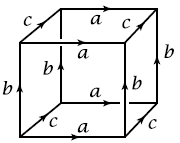
\includegraphics[scale=0.7]{izquierda}
\end{figure}

Como complejo celular hay una 3-célula, tres 2-células (contadas en el cociente, aunque en el dibujo parezcan 6), tres 1-células y una 1-célula. Ahora el complejo de cadenas es
\[
0\to Z\xrightarrow{d_3}\Z\oplus\Z\oplus\Z\xrightarrow{d_2}\Z\oplus\Z\oplus\Z\xrightarrow{d_1}\Z\to 0
\]
De nuevo $H_0(T^3)=\Z$ y $d_1=0$. También tenemos que $d_2=0$ porque sobre cada 2-célula se comporta como el pegamiento para el toro $M_2$. Vamos a probar que $d_3$ también es 0. Consideremos el colapso a una de las caras, que llamamos $A$. La aplicación característica envía a una $S^2_A$ dos subespacios conexos de de $S^2$, uno en cada hemisferio, y envia lo restante a un punto (esto es lo que se correspondería con las otras caras $B$ y $C$). Denotamos $L$ y $R$ a los subespacios mencionados, que se mapean homeomórficamente a $S^2_A$. Fijamos que $L$ se mapea con grado 1. Entonces la aplicación $R\to S^2_A$ se puede expresar como una reflexión con respecto a un plano $R\to L$ seguida del homeomorfismo $L\to S^2_A$, con lo que tendría grado local $-1$. Con esto, $\deg(\Delta)=0$ y análogamente para el resto de las caras. Esto prueba que $d_3=0$. Por ello, $H_1(T^3)\cong H_2(T^3)\cong H_3(T^3)\cong \Z^3$ 
\end{ej}

\begin{ej}
Sea $K\times S^1$ tal como muestra la figura 

\begin{figure}[h!]
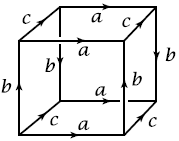
\includegraphics[scale=0.7]{derecha}
\end{figure}


Obtenemos $d_1=0$ de forma análoga al ejemplo anterior. En el caso de $d_2$, como $B$ y $C$ son toros, $d_2(B)=d_2(C)=0$. En cambio, $d_2(A)=2b$ por la orientación. Vemos ahora que pasa con $d_3$. Sobre $B$ y $C$ ocurre lo mismo que en el ejemplo anterior. Para $A$ volvemos a fijar el homeomorfismo $L\to S^2_A$ de grado 1. Para conseguir $R\to S^2_A$ basta rotar $L$ con respecto a un eje horizontal, que tien grado 1, con lo que el grado total es 2, así que $d_3=2C$. Tenemos entonces que $H_1(K\times S^1)=\Z_a\oplus \Z_b\oplus \Z_c/\gene{2b}\cong\Z\oplus\Z\oplus\Z/2\Z$ y $H_2(K\times S^1)=\Z_B\oplus\Z_C/\gene{2C}=\Z\oplus\Z/2\Z$. Por otra parte, $H_3(K\times S^1)=0$ porque $d_3$ es inyectivo.  
\end{ej}

\begin{ej}[Espacios de Moore]
Dado un grupo abeliano $G$, un espacio de Moore $M(n,G)$ es tal que $\widetilde{H}_i(M(n,G))=G$ si $i=n$ y 0 en cualquier otro caso. Sea $G=\Z_m$. Construimos $X=S^n\cup_{\phi}e^{n+1}$ con $\deg\phi=m$, lo cual sabemos que podemos hacerlo. El complejo de cadenas tiene $\Z$ en todas las dimensiones desde 0 hasta $n+1$ y 0 en el resto, siendo las aplicaciones borde todas nulas salvo la de dimensión más alta, que es multiplicación por $m$. Así que la homología es la que buscábamos.

Si $G$ es un grupo abeliano libre, basta tomar un wedge de $n$ copias de $S^n$. Por el teorema de estructuras, cualquier grupo abeliano finitamente presentado es unas una suma directa de grupos libres abelianos y grupos de torsión. Por tanto, para obtener un espacio de Moore con homología dada por un grupo abeliano finitamente generado, basta tomar wedge de los espacios que hemos visto, pues la homología reducida del wedge es la suma directa de las homologías. 

Si $G$ no es finitamente generado, entonces existe $F\to G$ donde $F$ es abeliano libre con base $\{x_\alpha\}_{\alpha\in I}$. Entonces $K=\ker(F\to G)$ es abeliano libre con base $\{y_{\beta}\}_{\beta\in J}$ por ser subgrupo de $F$ y además $G\cong F/K$. Podemos expresar $y_\beta=\sum_{\alpha}d_{\beta\alpha}x_\alpha$. Definimos el $n$-esqueleto $X^n=\bigvee_{\alpha\in I} S^n_{\alpha}$ y pegamos $e^{n+1}_{\beta}$ a $X^n$ siguiendo una aplicación $f_\beta:S^n_{\beta}\to X^n$ tal que $\deg(\Delta_{\beta\alpha})=\deg(f_{\beta})|_{\alpha}=d_{\beta\alpha}$. También hay que definir $X^0$, que lo hacemos como una sola 0-célula (el resto son vacíos). Tenemos entonces $d_{n+1}:\oplus_{\beta}\Z=K\to \oplus_{\alpha}\Z=F$ definida como $y_\beta\mapsto \sum_{\alpha}d_{\beta\alpha}$, que es claramente inyectiva. Así que que $\widetilde{H}_q(X)=G$ si $q=n$ y 0 en otro caso. 

Esta contrucción también sirve para generar aplicaciones de grado arbitrario. Dado $\beta$, $S^n_{\beta}$ y elegidas $\sum_{\alpha}|d_{\alpha\beta}|$ discos abiertos disjuntos sobre $S^n_{\beta}$, enviamos el complementario de estos discos al puntos wedge de $\bigvee_\alpha S^n_{\alpha}$ y sobre cada $S^n_{\alpha}$ enviamos $|d_{\beta\alpha}|$ discos mediante homeomorfismo de grado 1 si $d_{\alpha\beta}>0$ y de grado $-1$ si $d_{\alpha\beta}<0$ (o mantener las de grado 1 y componer al final con una reflexión).

También podemos construir un espacio $M=M(G_{i_1},\dots, G_{i_n})$ tal que $\widetilde{H}_q(M)=G_{i_j}$ si $q=i_j$ y 0 en caso contrario. Para ello basta hacer wedge de los anteriores.
\end{ej}

\begin{ej}[Espacios de lentes]
Dado un entero $m>1$, construimos espacios $L_m(l_1,\dots, l_n)$ donde $l_i\leq m$ son enteros tales que $\gcd(l_i,m)=1$. Algunos de estos espacios nos darán ejemplos de espacios homotópicamente equivalentes que no son homeomorfos porque no son equivalentes mediante homotopía \emph{simple} (homotopía de colapsos como en complejos simpliciales pero en CW-complejos). Sea $\Z_m$ actuando sobre $S^{2n-1}\subseteq\C^n$ mediante la rotación $\rho(z_1,\dots, z_n)=(e^{2\pi il_1/m}z_1,\dots, e^{2\pi il_n/m}z_n)$ en cada coordenada $z_j$, es decir, una rotación de ángulo $2\pi l_j/m$. Como $\gcd(l_j,m)=1$, la acción de $\rho$ es libre. Se puede probar que $S^{2n-1}=S^1*\cdots S^1$ ($n$ veces el joint) y en general por indución $S^n*S^m=S^{n+m+1}$, así que podemos interpretar la rotación como una rotación en cada $S^1$ sobre un segmento. Definimos $L_m(l_1,\dots, l_n)$ como $S^{2m-1}/\Z_m$. Veremos que el espacio de lentes tiene una estructura de CW-complejo con una célula en cada dimensión hasta $2n-1$ y aplicaciones borde $d_=0$ para $k$ impar y multiplicación por $m$ para $k$ par. Esto nos da la homología 
$$H_k(L_m(l_1,\dots, l_n))=\begin{cases}
\Z & k=0,2n-1\\
\Z_m & k\text{ impar } 0<k<2n-1\\
0 & c.c
\end{cases}$$

Para obtener la estructura de CW complejo, empezamos tomando vértices en $S^1$ definidos $v_j=e^{2\pi i j/m}$ para $j=1,\dots, m-1$ y segmentos entre los vértices, que denotamos $I_j=[v_j,v_{j+1}]$. En el hiperplano $\C^{n-1}$ tenemos $S^{n-3}$ perpendicular a $S^1$ donde suponemos que ya hemos dotado de estructura (habría que hacerlo inductivamente, pero para $S^0$ y $S^1$ es trivial). Podemos hacer el joint (que va a ser un cono) $v_j*S^{2n-3}=B_j^{2n-2}$ y el joint $I_j*S^{2n-3}=B_j^{2n-1}$. Con esto tenemos cubierta la esfera $S^{2n-1}$ (ver figura \ref{lens}).  


Se comprueba que $\rho$ lleva $S^{2n-3}$ en sí misma y rota $S^1\subseteq \C$ por un giro de ángulo $2\pi l_n/m$, luego $\rho$ permuta $B^{2n-2}$ y $B^{2n-1}_j$ entre sí. Como $l_n$ es primo con $m$, existe $r$ tal que $rl_n\equiv 1\mod m$, luego $\rho^r$ tiene orden $m$ y generará $\Z_m$ (sobre $S^1$). Además $\rho^r(B_j^{2n-2}=B_{j+1}^{2n-2}$ y $\rho^r(B_j^{2n-1})=B_{j+1}^{2n-1}$. Concluimos que $\rho^r$ permuta las $(2n-1)$-células y las $(2n-2)$-células entre sí, por lo que existe una única $(2n-1)$-célula y una única $(2n-2)$-célula en $L_m(l_1,\dots, l_m)=S^{2n-1}/\Z_m$. 

\begin{figure}[h!]
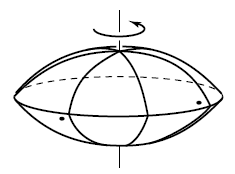
\includegraphics[scale=0.7]{lens}
\caption{Ejemplo donde en el plano tenemos $S^1$ y $S^{2n-3}=S^0$ está situada en el eje vertical, con lo que unimos $S^0$ a cada vértice $v_j$.}\label{lens}
\end{figure}


Veamos ahora que las diferenciales son las que decíamos. Tenemos que ver el grado de la la aplicación $S^{2n-2}\to X^{2n-2}\to X^{2n-2}/X^{2n-1}=S^{2n-2}_{e^{2n-1}}$. Para pasar de $B_j$ a $B_{j+1}$ hay que hacer una reflexión, y en el cociente la diferencia es una rotación, por lo que el grado local de un $B_j$ se cancela con el de $B_{j+1}$, obteniendo $d_{2n-1}=0$. 

Vemos el grado ahora de $S^{2n-3}\to X^{2n-3}=S^{2n-3}/\Z_m\to S^{2n-3}=L_m^{2n-3}/L_m^{2n-4}$. Observamos que la aplicación de pegamiento es la identidad en $S^{2n-3}$. Como inductivamente habíamos dividido $S^{2n-3}$ en $m$ células que se identifican en el cociente, hay $m$ preimágenes de grado 1, así que $d_{2n-2}=m$. 

Inductivamente se deducen el de $d_k$ en dimensiones inferiores.
\end{ej}


\section{Suciones de Mayer-Vietoris}
\begin{teorema}
Dado un espacio $X$ y $A,B\subseteq X$ subespacios cuyos interiores recubren $X$, entonces hay una sucesióne xacta larga
\[
\cdots\to H_n(A\cap B)\to H_n(A)\oplus H_n(B)\to H_n(X)\to H_{n-1}(A\cap B)\to\cdots
\]
\end{teorema}
\begin{dem}
 Tomamos $\UU=\{A,B\}$, y por el lema \ref{peque}, $C^{\UU}_*(X)\hookrightarrow C_*(X)$ induce isomorfismo en homología. Vemos que tenemos una sucesión exacta corta de complejos de cadenas
 \[
 0\to C_*(A\cap B)\to C_*(A)\oplus C_*(B)\to C_*^{\UU}(X)\to 0
 \]
La primera aplicación no nula viene dada por $((i_1)_\sharp, (i_2)_\sharp)$ donde $i_1:A\cap B\hookrightarrow A$, $i_2:A\cap B\hookrightarrow B$, que es claramente inyectiva. La segunda aplicación viene dada por $(j_1)_\sharp-(j_2)_\sharp$, donde $j_1:A\hookrightarrow X$, $j_2:B\hookrightarrow X$, que es sobreyectiva porque $C_*^{\UU}(X)$ es el complejo subordinado a $\UU$, luego los símplices singulares están contenidos en $A$ o en $B$. La exactitud es sencilla porque $j_1i_1=j_2i_2$, y además si $(j_1)_\sharp(x)-(j_2)_\sharp(y)=0$, entonces $(j_1)_\sharp(x)=(j_2)_\sharp(y)$, entonces $x=y$ ya demás $x\in A\cap B$ (dos simplices singulares en el complejo subordinados son iguales si y solo si tienen los mismo coeficientes y están en el mismo conjunto), por lo que está en la imagen de $C_*(A\cap B)$. De esta sucesión exacta corta se deriva la larga de la forma habitual.
\end{dem}

\begin{nota}
El teorema también es cierto si $X$ es un $CW$-complejo y $A,B\subseteq X$ son subcomplejos tales que $X=A\cup B$, porque hay abiertos $U_A$ y $U_B$ que contienen respectivamente a $A$ y $B$ como retracto de deformación y tales que $A\cap B\subseteq U_A\cap U_B$ también como retracto de deformación. Para verlo, si consideramos una celda de $X$ pegada a $A$, basta tomar una corona abierta de esa celda y unirla a $A$, que se puede retraer sobre $A$. Esto también podemos hacerlo en $B$, con lo cual también se hace sobre la intersección. 
\end{nota}

La sucesión de Mayer-Vietoris también tiene una versión reducida aumentando con $\Z\xrightarrow{\binom{1}{1}}\Z\oplus\Z\xrightarrow{(1,-1)}\Z\to 0$. 


\begin{ej}
Sea $K$ la botella de Klein expresada como unión de dos bandas de Möbius $M_1$ y $M_2$, que podemos consideraras como subcomplejos de $K$. Aplicamos Mayer-Vietoris reducida. Tenemos que $M_1\cap M_2\cong S^1\simeq M_1\simeq M_2$. Tenemos entonces la sucesión exacta
\[
0\to H_2(K)\to H_1(M_1\cap M_2)=\Z\xrightarrow{i_*} H_1(M_1)\oplus H_1(M_2)=\Z\oplus \Z\to H_1(K)\to 0
\]
El generador de $M_1\cap M_2$ está dado por la circunferencia del borde de la banda, que es homólogo a recorrer 2 veces la circunferencia central (una por arriba y otra por abajo), que es la que genera cada $H_1(M_i)$, por lo que $i_*(1)=(2,-2)$. Como $i_*$ es inyectivo, la exactitud nos da $H_2(K)=0$. Obtenemos también que $H_1(K)=\Z\oplus\Z/\gene{(2,-2)}\cong \Z\oplus \Z_2$. 
\end{ej}

\begin{ej}
Sean $f,g:X\to Y$ y hacemos el cociente $Z=(X\times I)\sqcup Y/\sim$ por la relación $(x,0)\sim f(x), (x,1)\sim g(x)$. Consideramos las sucesines de homología de los pares $(X\times I,X\times\partial I)$ y $(Z,Y)$, que conmutan mediante la aplciación $q$ de paso al cociente.
\[
\begin{tikzcd}
H_{n+1}(X\times I,X\times\partial I)\arrow[r,"\Delta"]\arrow[d, "q_*"] & H_n(X\times\partial I)\arrow[r]\arrow[d, "q_*"] & H_n(X\times I)\arrow[r]\arrow[d, "q_*"] & H_n(X\times I,X\times\partial I)\arrow[d, "q_*"]\\
 H_{n+1}(Z,Y)\arrow[r,"\Delta"] & H_n(Y)\arrow[r] & H_n(Z)\arrow[r] & H_n(Z,Y)
\end{tikzcd}
\]




Ahora, $X\times I\simeq X\times\{0\}$, por lo que $i_*$ es sobreyectiva. Eso quiere decir que $\Delta$ es inyectivo, porque el resto de aplicaciones son 0. Además, $\ker i_*\subseteq H_n(X\times\{0\})\oplus H_n(X\times\{1\})$ consiste en los pares $([\alpha],-[\alpha])$, que es un grupo isomorfo a $H_n(X)$ porque todas sus clases están representadas.  Por tanto. $H_{n+1}(X\times I,X\times\partial I)\cong H_n(X)$. 

Dada una clase $[z]\in H_n(X)$, por el isomorfismo que hemos dado antes, $\Delta([z])=([\alpha],-[\alpha])$, que en el cociente se identifica con $f^*\alpha-g^*\alpha$, por lo que $q_*\Delta=f_*-g_*$. Todas las parejas que estamos considerando son buenas parejas, por lo que $\widetilde{H}_{n+1}(X\times I/X\times\partial I)\cong H_{n+1}(X\times I,X\times\partial I)\underset{q_*}{\cong} \widetilde{H}_n(Z/Y)\cong \widetilde{H}_{n+1}(Z/Y)$. 

Deducimos entonces $H_{n+1}(Z,Y)\cong H_n(X)$. Obtenemos entonces la sucesión exacta larga
\[
\cdots H_n(X)\xrightarrow{f_*-g_*}H_n(Y)\xrightarrow{i_*} H_n(Z)\to H_{n-1}(X)\to\cdots
\]
Esto es una generalización de Mayer-Vietoris en el siguiente sentido: Consideramos las inclusiones $f:A\cap B\to A\to A\sqcup B$ y $g:A\cap B\to B\to A\sqcup B$ como en Mayer-Vietoris. La anterior sucesión exacta se traduce entonces como
\[
H_n(A\cap B)\xrightarrow{i_*} H_n(A)\oplus H_n(B)\to H_n(A\cup B)
\]
\end{ej}



\section{Homología con coeficientes}
Sea $G$ un grupo abeliano con notación aditiva. El complejo de cadenas singulares de un espacio $X$ con coeficientes en $G$ se define como $C_*(X;G)=\{\sum_{\sigma:\Delta^n}\to X g_{\sigma}\sigma\mid g\in G$ casi todos nulos$\}$, que es un grupo abeliano sumando coeficiente a coeficiente. En particular $C_n(X)=C_n(X;\Z)$. La diferencial se define exactamente igual, ya que multiplicar por 1 es dejarlo igual y multiplicar por $-1$ es tomar el opuesto. Así que la homología con coeficientes en $G$ es simplemente $H_n(X;G)=H_n(C_*(X;G))$. Se puede definir el complejo de cadenas como $C_n(X)\otimes_{\Z}G$, con la diferencial $d\otimes Id_G$, siendo $d$ la diferencial usual. Sin embargo $H_n(X;G)\not\cong H_n(X)\otimes_{\Z}G$ porque el producto tensorial no respeta sucesiones exactas ni núcleos. 

 También existe la homología relativa del par $(X,A)$ con coeficientes en $G$ denotada $H_n(X,A;G)$ de forma absolutamente análoga. El complejo aumentado se puede construir con $C_0(X;G)\xrightarrow{\varepsilon}G\to 0$ con $\varepsilon$ definido como suma de los coeficientes, por lo que también tenemos la homología reducida $\widetilde{H}_n(X;G)$. Todos los resultados que hemos visto para homología en $\Z$ se tienen con coeficientes en $G$ con las mismas pruebas.
 
 \begin{ej}
 Calculamos $\widetilde{H}_*(S^n;G)$ por inducción en $n$. Para $n=0$, $\widetilde{H}_0(S^0;G)=G$ y 0 para el resto. Suponemos que $\widetilde{H}_n(S^n;G)=G$ y para cualquier otro grado es 0. Consideramos ahora el par $(D^{n+1}, S^n)$. Como $(D^{n+1}, S^n)$ es un buen par, $\widetilde{H}_{m+1}(D^{n+1},S^n;G)\cong \widetilde{H}_{m+1}(S^{n+1};G)$, y la sucesión de homología relativa reducida del par nos da $\widetilde{H}_{m+1}(D^{n+1},S^n;G)\cong \widetilde{H}_m(S^n;G)$. 
 \end{ej}
 Si $X$ es un CW-complejo, se puede definir $C_n^{CW}(X;G)=H_n(X^n,X^{n-1};G)$, que ahora es el grupo formado por las combinaciones con coeficientes en $G$ de las $n$-células de $X$ (identificamos cada célula con su aplicación característica). La definición de la diferencial es análoga, y tendríamos lo siguiente, donde $d'$ denota la diferencial para el caso entero
 \[
 d(\sum_\alpha g_\alpha e_{\alpha}^n)=\sum_{\alpha}g_\alpha d'(e_{\alpha}^n)=\sum_{\alpha}g_\alpha(\sum_{\beta}n_{\alpha\beta}e_{\beta}^{n-1})=\sum_{\alpha,\beta}(g_\alpha n_{\alpha\beta})e^{n-1}_{\beta}
 \]
 
Un homomorfismo de grupos abelianos $\varphi:G\to H$  induce $\varphi_\sharp:C_*(X;G)\to C_*(X;H)$, simplemente sustituyendo cada coeficiente por su imagen mediante $\varphi$, con lo que se induce $\varphi_*:H_*(X;G)\to H_*(X;H)$ con la misma functorialidad y naturalidad con respecto a las aplicaciones inducidas por $f:X\to Y$ de las aplicaciones inducidas habituales, es decir, conmutas los diagramas de la forma
\[
\begin{tikzcd}
C_*(X;G)\arrow[r, "\varphi_\sharp"]\arrow[d, "f_\sharp"] & C_*(X;H)\arrow[d, "f_\sharp"]\\
C_*(Y;G)\arrow[r, "\varphi_\sharp"] & C_*(Y;H)
\end{tikzcd}
\]
y esta conmutatividad se transmite a la homología.
 
 \begin{prop}
 Dada $f:S^n\to S^n$, la aplicación inducida $f_*:\widetilde{H}_n(S^n;G)\to\widetilde{H}_n(S^n;G)$ es la multiplicacón por $\deg(f)$. 
 \end{prop}
\begin{dem}
Fijado $g\in G$, tomamos el homomorfismo $\widetilde{H}_n(S^n,\Z)=\Z to G=\widetilde{H}_n(S^n;G)$ dado por $1\mapsto g$. Tenemos el diagrama conmutativo
\[
\begin{tikzcd}
\Z=\widetilde{H}_n(S^n;\Z)\arrow[r, "f_*=\deg(f)"]\arrow[d, "\varphi_*"] & \widetilde{H}_n(S^n;\Z)=\Z\arrow[d, "\varphi_*"]\\
G=\widetilde{H}_n(S^n;G)\arrow[r, "f_*"] &\widetilde{H}_n(S^n;G)
\end{tikzcd}
\]
de donde se deduce el resultado.
\end{dem}


\begin{ej}
Sea $X=\R P^{\infty}$, con $C_n^{CW}=G$ para todo $n$. Las diferenciales son iguales que en el caso de $\Z$, entiendiendo la multiplicación por 2 como sumar un elemento consigo mismo. Si tomamos $G=\Z_2$, la multiplicación por 2 es el homomorfismo nulo, por lo que $H_*(\R P^{\infty};\Z_2)$ es isomorfo al complejo de cadenas. Si tomamos $G$ un cuerpo ($\Q$ o $\R$ por ejemplo), la multiplicación por 2 es isomorfismo, con lo que la homología es 0 en todos los grados salvo en 0, que es igual a $G$. 
\end{ej}


\section{Característica de Euler}
\begin{defi}
Sea $X$ un CW-complejo finito. Se define la característica de Euler de $X$ como $\chi(X)=\sum_{n\geq 0}(-1)^nc_n$, donde $c_n$ es el número de $n$-células de $X$. Se tiene que $c_n=rg(C_n^{CW}(X))=rg(H_n(X^n,X^{n-1})$ como grupo abeliano libre finitamente generado. 
\end{defi}
\begin{nota}
El rango de un grupo abeliano finitamente $G$ generado se puede definir como la dimensión del $\Q$-espacio vectorial $G\otimes_{\Z} G$, porque esto elimina la parte de torsión.
\end{nota}

\begin{prop}
Si $0\to A\to B\to C\to 0$ es una sucesión exacta corta de grupos abelianos finitamente generados, entonces $rg(B)=rg(A)+rg(C)$.
\end{prop}
Esta proposición se puede probar haciendo producto tensorial por $\Q$, porque aunque el producto tensorial en general no es exacto, al hacerlo por $\Q$ sí. Existen otras pruebas más elementales pero más costosas. Podemos aplicar esto a las sucesiones exactas
\[
0\to B_n\to Z_n\to H_n\to 0
\]
\[
0\to Z_n\to C_n\to B_{n-1}\to 0
\]
De la primera, $rg(Z_n)=rg(B_n)+rg(H_n)$ y de la segunda $rg(C_n)=rg(Z_n)+rg(B_{n-1})$. Sustituyendo obtenemos $rg(C_n)=rg(B_n)+rg(H_n)+rg(B_{n-1})$. De aquí deducimos que $\chi(X)=\sum_{n\geq 0}(-1)^nrg(C_n)$. 

\begin{ej}
$\chi(M_g)=1-2g+1=2-2g$, $\chi(N_g)=0-(g-1)+1=2-g$. 
\end{ej}

\section{Propiedad de Extensión de Homotopía y CW-complejos}


\begin{defi}
Diremos que $(X,A)$ verifica la \emph{propiedad de extensión de homotopía} (HEP) si dadas $f:X\to Y$ y $H:A\times I\to Y$ con $H_0=f|_{A}$, entonces existe $K:X\times I$ tal que $K|_{A\times I}=H$.
\[
\begin{tikzcd}
X\times\{0\}\sqcup A\times I\arrow[r, hookrightarrow]\arrow[d, bend left, shift left=5, end anchor={[xshift=-7]}, start anchor={[yshift=2]},  "H"]\arrow[d, bend right, shift right,"f"] & X\times I\arrow[dl, bend left, dashed, "K"]\\
Y &
\end{tikzcd}
\]

\begin{figure}[h!]
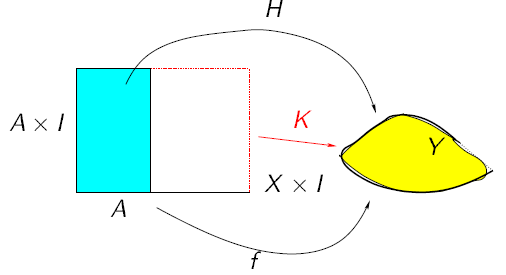
\includegraphics[scale=0.6]{HEP}
\end{figure}
\end{defi}

\begin{prop}
Una pareja $(X,A)$ verifica la HEP si y solo si $X\times\{0\}\cup A\times I$ es retracto de deformación fuerte de $X\times I$. 
\end{prop}
El resultado es cierto en general (ver apéndice de Hatcher, proposición A.18), aunque asumiendo $A$ cerrado es fácil

\[
\begin{tikzcd}[column sep=tiny]
Y=X\times\{0\}\sqcup A\times I\arrow[dd, "Id"']\arrow[dr, hookrightarrow] & & & X\times\{0\}\sqcup A\times I\arrow[dd, "Id"']\arrow[dr, hookrightarrow]& &\\
& X\times I\arrow[dr, dashed, "K=r"] & & & X\times I\arrow[ dl, "r"']\arrow[dr, dashed, "K"] &\\
X\times\{0\}\cup A\times I\arrow[rr, "Id_X\cup Id_{A\times I}"'] & &Y & X\times\{0\}\cup A\times I\arrow[rr, "f\cup H"'] & &Y
\end{tikzcd}
\]
Al ser la intersección de los dominios de las funciones de abajo cerrados, se puede hacer la unión de forma continua. A la izquierda estamos suponiendo que $(X,A)$ verifica la HEP y a la derecha la implicación recíproca. 


\begin{coro}
Si $(X,A)$ tiene la HEP, entonces $(X\times Z, A\times Z)$ también la tiene.
\end{coro}

\begin{coro}
Si $(X,A)$ tiene la HEP y $X$ es Hausdorff, entonces $A$ es cerrado en $X$. 
\end{coro}
Este corolario se tiene porque si $X$ es Hausdorff, entonces $X\times I$ lo es, y entonces cualquier retracto de deformación fuerte suyo es cerrado. Otra idea es que si $X$ es Hausdorff entonces $X\times I$ también, y  entonces la diagonal $\Delta\subseteq (X\times I)\times(X\times I)$ también lo es. Se puede definir $f=(r,Id):X\times I\to  (X\times I)\times(X\times I)$, de modo que $f^{-1}(\Delta)=\{(x,t)\mid r(x,t)=(x,t)\}=X\times\{0\}\cup A\times I\subseteq X\times I$ es cerrado. La intersección de este espacio con $X\times\{1/2\}$ es cerrada y homeomorfa a $A$, por lo que $A$ es cerrado. 

\begin{ej}
\definecolor{qqffqq}{rgb}{0.,1.,0.}
\begin{tikzpicture}[line cap=round,line join=round,>=triangle 45,x=1.0cm,y=1.0cm]
\clip(-2.6426666666666674,-0.7) rectangle (8.952,3.05333333333333);
\fill[line width=2.pt,color=qqffqq,fill=qqffqq,fill opacity=0.10000000149011612] (0.,0.) -- (5.,0.) -- (5.,3.) -- (0.,3.) -- cycle;
\draw [line width=2.pt,color=qqffqq] (0.,0.)-- (5.,0.);
\draw [line width=2.pt,color=qqffqq] (5.,0.)-- (5.,3.);
\draw [line width=2.pt,color=qqffqq] (5.,3.)-- (0.,3.);
\draw [line width=2.pt,color=qqffqq] (0.,3.)-- (0.,0.);
\draw [line width=2.pt] (0.,3.)-- (0.,0.);
\draw [line width=2.pt] (5.,3.)-- (5.,0.);
\draw [line width=2.pt] (2.4933333333333336,0.)-- (2.506666666666667,3.);
\draw [line width=2.pt] (1.3066666666666666,0.)-- (1.3066666666666666,3.);
\draw [line width=2.pt] (0.6,0.)-- (0.6,3.);
\draw (4.9093333333333335,0.028) node[anchor=north west] {$1$};
\draw (2.4133333333333336,0.0813333333333357) node[anchor=north west] {$\frac{1}{2}$};
\draw (0.5253333333333331,0.10266666666666902) node[anchor=north west] {$\frac{1}{8}$};
\draw (1.2186666666666666,0.10266666666666902) node[anchor=north west] {$\frac{1}{4}$};
\draw (-0.5,0.04933333333333573) node[anchor=north west] {$0$};
\draw (-2.7,1.852) node[anchor=north west] {$(X\times I, A\times I)$};
\begin{scriptsize}
\draw [fill=black] (0.12,1.5) circle (1.0pt);
\draw [fill=black] (0.40444444444444444,1.4928888888888896) circle (1.0pt);
\draw [fill=black] (0.26222222222222225,1.4928888888888896) circle (1.0pt);
\draw [fill=black] (0.2977777777777778,-0.2422222222222205) circle (1.0pt);
\draw [fill=black] (0.46133333333333343,-0.2422222222222205) circle (1.0pt);
\draw [fill=black] (0.10933333333333305,-0.24933333333333138) circle (1.0pt);
\end{scriptsize}
\end{tikzpicture}

Como $X\times\{0\}\cup A\times I$ no es retracto de deformación fuerte de $X\times I$, este par no cumple la HEP.
\end{ej}


\subsection{Mapping Cylinder Neighborhood}
\begin{defi}
El cilindro de una aplicación (mapping cylinder) $f:X\to Y$ es el espacio $M_f=(([0,1]\times X)\cup Y)/sim$ donde la relación de equivalencia está generada por $(0,x)\sim f(x)$. 
\end{defi}

\begin{prop}
Si $A$ tiene un entorno que es un cilindro de una aplicación, entonces $(X,A)$ tiene la HEP. 
\end{prop}

Sea $(N,B)\subseteq X$ un entorno cerrado de $A$ tal que $N-B$ es entorno abierto de $A$, existe $f:B\to A$ y $(N;A,B)\cong_h (M_f;A,B)$ son homeomorfos con $h|_A=Id_A$ y $h|_B=Id_B$. 

Tenemos la retracción $r:I\times I\to I\times\{0\}\cup \partial I\times I$, por lo que $(I\times I,\partial I\times I)$ tiene la HEP, porlo que también se sigue teniendo al multiplicar por $B$, lo que nos da $Id_B\times r:B\times I\times I\to B\times(I\times \{0\}\cup\partial I\times I)$. Esta aplicación induce otra en el cociente $M_f\times I=(B\times I\cup_f A)\times I\to M_f\times\{0\}\cup(A\cup B)\times I$. Así, $(M_f,A\cup B)$ tiene la HEP, y por tanto, $(N,A\cup B)$ también.

\begin{figure}[h!]
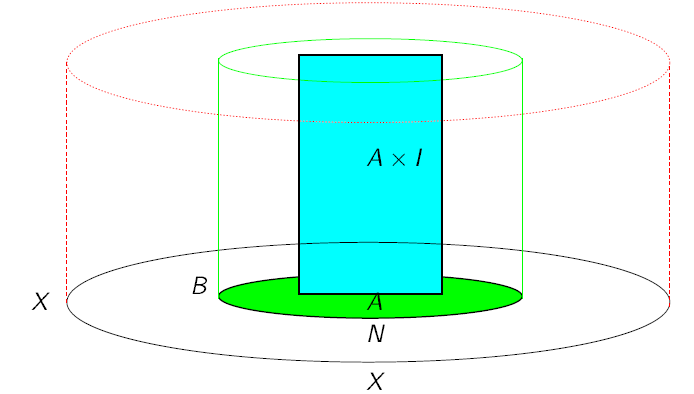
\includegraphics[scale=0.5]{mpc}
\end{figure}

\begin{prop}
Si $(X,A)$ es una pareja de CW-complejos, entonces tienen la HEP. 
\end{prop}
\begin{dem}
Como $D^n\times I$ se retrae sobre $D^n\times\{0\}\cup\partial D^n\times I$, entonces para cada $n$ existen retracciones 
\[
\begin{tikzcd}
X^n\times I=X^n\times\{0\}\cup (X^{n-1}\cup A)\times I\cup_{\sqcup \partial D^n\times I}(\sqcup D^n\times I)\arrow[d, "r_n"]\\
X^n\times\{0\}\cup (X^{n-1}\cup A)\times I
\end{tikzcd}
\]
Obtenemos una retracción $r:X\times I \to X\times\{0\}\cup A\times I$ ensamblando $r_n$ reparametrizada en $\left[\frac{1}{2^{n+1}},\frac{1}{2^{n}}\right]$.
\end{dem}

\begin{prop}
Si $(X,A)$ tiene la HEP y $A$ es contráctil, entonces $q:X\to X/A$ es una equivalencia de homotopía. 
\end{prop}
\begin{dem}
Dada la contracción $h:A\times I\to A$ con $h_0=Id_A$ y $h_1=c_*$ y, usando HEP, tenemos
\[
\begin{tikzcd}
X\times\{0\}\cup A\times I\arrow[r, "Id\cup h"]\arrow[d, hookrightarrow] & X\times I\arrow[r, "q\times Id"] & X/A\times I\\
X\times I\arrow[ur, dashed, "F=\{f_t\}"] \arrow[r, "q\times Id"]& X/A\times I\arrow[ur, dashed, "\overline{F}=\{\overline{f}_t\}"]
\end{tikzcd}
\]
Ahora, $f_1(A)=*$ induce $g:X/A\to X$.
\[
\begin{tikzcd}
X\arrow[r, "f_1"]\arrow[d, "q"'] \arrow[dr, phantom, "(1)", very near start] & X\arrow[d, "q"]\\
X/A\arrow[ur, dashed, "g"]\arrow[r,"\overline{f}_1"'] & X/A\arrow[ul, phantom, "(2)", very near start]{tiny} 
\end{tikzcd}
\]
Como $(1)$ conmuta, $qg([x])=qgq(x)=qf_1(x)=\overline{f}_1q(x)=\overline{f}_1([x])$, por lo que $(2)$ conmuta. Así, $qg=f_1\simeq_F f_0=Id_X$; $qg=\overline{f}_1\simeq_{\overline{F}}\overline{f}_0=Id_{X/A}$, luego $q$ y $g$ son equivalencias de homotopía. 
\end{dem}

\begin{prop}
Si $(X,A)$ es una pareja de CW-complejos y $f\simeq g:A\to X_0$, entonces $X\cup_f X_0$ y $X\cup_g X_0$ son homotópicamente equivalentes. 
\end{prop}
\begin{dem}
Sea $F:A\times I\to X_0$ la homotopía $F_0=f\simeq g=F_1$. Consideramos el pushout
\[
\begin{tikzcd}
A\times I\arrow[d,hookrightarrow]\arrow[r, "F"] & X_0\arrow[d]\\
X\times I\arrow[r] & X_0\cup_F (X\times I)
\end{tikzcd}
\]
que contiene a $X_0\cup_f X$ y a $X_0\cup_g X$.

\begin{figure}[h!]
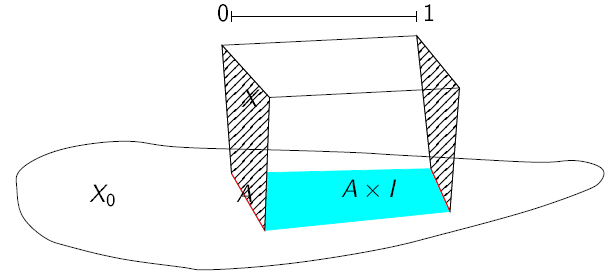
\includegraphics[scale=0.5]{retract}
\end{figure}

$X\times I$ se retrae sobre $X\times\{0\}\cup A\times I$ y también sobre $X\times\{1\}\cup A\times I$ por ser CW-complejos. Por tanto, $X_0\cup_F(X\times I)$ se retrae tanto sobre $X_0\cup_f X$ como sobre $X_0\cup_g X$, luego son homotópicamente equivalente relativos a $A$.
\end{dem}

\begin{prop}
Si $(X,A)$ e $(Y,A)$ son parejas de CW-complejos y $f:X\to Y$ es una equivalencia de homotopía con $f|_{A}=Id_A$, entonces $f$ es equivalencia de homotopía relativa a $A$.
\end{prop}
\begin{dem}
Tenemos $f:X\to Y$ con $A\subseteq X\cap Y$ y $f|_{A}=Id_A$. Dada $g:Y\to X$ con $gf\simeq_H Id_X$, aplicamos la HEP y obtenemos $g_1:Y\to X$ con la extensión $G$ de $H$. 

\begin{figure}[h!]
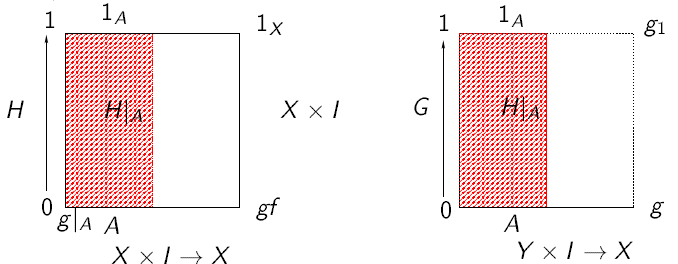
\includegraphics[scale=0.6]{extension}
\end{figure}
Obtenemos una homotopía $K:g_1f\simeq Id_X: X\times I\to X$. Denotamos con signo menos recorrer el intervalo $[0,1]$ en sentido contrario (ver figuras).

\begin{figure}[h!]
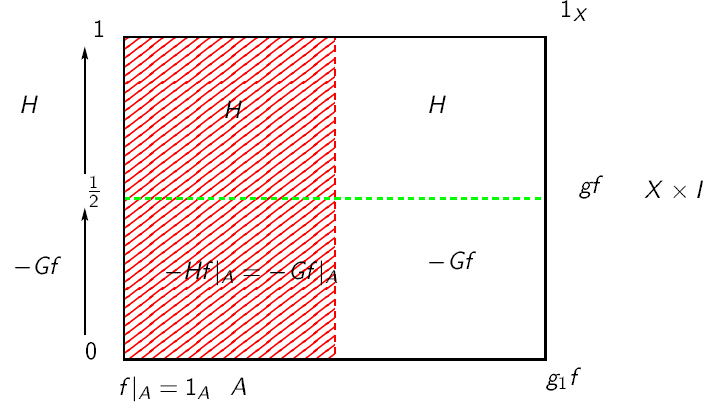
\includegraphics[scale=0.6]{k}
\end{figure}

Nótese que sobre $A$, $K_t=K_{1-t}$. Modificamos la homotopía $K$ sobre $A$ con un \emph{track} (2-homotopía, homotopía de homotopía) $\widehat{K}:A\times I\times I\to X$.

\begin{figure}[h!]
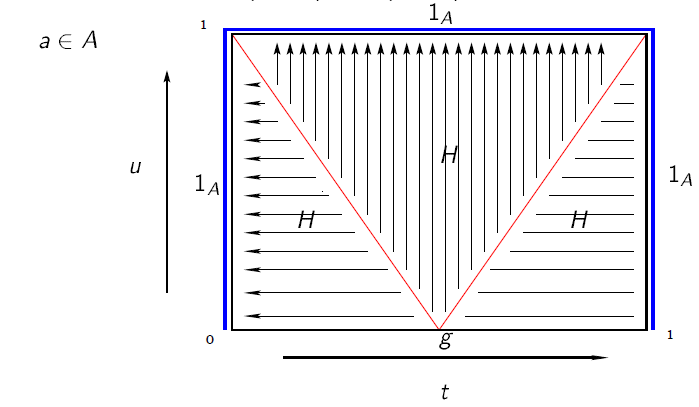
\includegraphics[scale=0.5]{tilde}
\end{figure}

Aplicamos la HEP a $(X\times I, A\times I)$ y obtenemos $g_1f\simeq Id_X\ rel\ A$. 
\begin{figure}[h!]
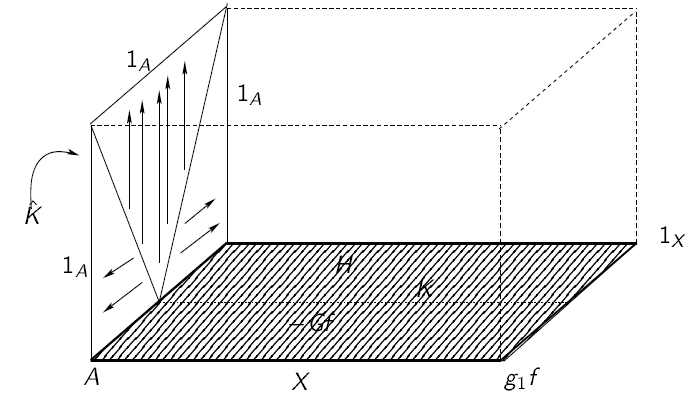
\includegraphics[scale=0.5]{rel}
\end{figure}

Como $g_1\simeq g$, entonces $fg_1\simeq fg\simeq Id_Y$. Es decir, $fg_1\simeq Id_Y$ y $g_1|_{A}=Id_A$. Podemos pues aplicar el proceso anterior a $g_1$, obteniendo $f_1:X\to Y$ con $f_1|_{A}=Id_A$ verificando $f_1g_1\simeq Id_A\ rel\ A$. Ahora, $f_1\simeq f_1(g_1g)=(f_1g_1)f\simeq f\ rel A$ y entonces $fg_1\simeq_{rel\ A}f_1g_1\simeq_{rel\ A}Id_Y$. 
\end{dem}


\begin{coro}
Si $(X,A)$ tiene la HEP y $A\hookrightarrow X$ es una equivalencia de homotopía, entonces $A$ es retracto de deformación fuerte de $X$. 
\end{coro}
\begin{coro}
Una aplicación $f:X\to Y$ es una equivalencia de homotopía si y solo si $X$ es retracto de deformación fuerte de $M_f$. Así, $X$ e $Y$ son homotópicamente equivalentes si y solo si existe $Z\supseteq X,Y$ teniéndolos como retractos de deformación fuerte.
\end{coro}
\begin{dem}
Tenemos 
\[
\begin{tikzcd}[row sep=28]
X\arrow[r, "f"] \arrow[dr, hookrightarrow, "i"']& Y\arrow[d, bend right, "j"']\\
& M_f\arrow[u, bend right, "r"']
\end{tikzcd}
\]
Como $r$ y $j$ son equivalencias de homotopías, $f=ri$ y $i\simeq jf$, entonces $f$ es equivalencia de homotopía si y solo si $i$ lo es. Como $X$ tiene un entorno cilíndrico en $M_f$, por ejemplo $X\times[0,1/3)$, $(M_f,X)$ tiene la HEP y como $X\hookrightarrow M_f$ es equivalencia de homotopía, entonces por el corolario anterior es retracto de deformación. 
\end{dem}


\section{Axiomas en homología}
Una \emph{teoría de homología reducida} es una familia de functores covariantes $\tilde{h}_*=\{\tilde{h}_n\}_{n\in\Z}:CW\to Ab$ satisfaciendo los siguientes axiomas
\begin{enumerate}
\item si $f\simeq g$, entonces $\tilde{h}_*(f)=f_*=g_*=\tilde{h}_*(g)$;
\item existen transformaciones naturales $\partial:\tilde{h}_n(X/A)\to\tilde{h}_{n-1}(A)$ tal que para parejas $(X,A)$ de CW se obtiene una sucesión exacta larga
\[
\cdots\to \tilde{h}_n(X)\xrightarrow{q_*}\tilde{h}_n(X/A)\xrightarrow{\partial}\tilde{h}_{n-1}(A)\xrightarrow{i_*}\tilde{h}_{n-1}(X)\to\cdots
\]
\item si $X=\bigvee_\alpha X_\alpha$ entonces las inclusiones $i_\alpha:X_\alpha\to X$ inducen isomorfismos $$\oplus_\alpha i_{\alpha*}:\oplus_\alpha\tilde{h}_n(X_\alpha)\to \tilde{h}_n(X).$$

\end{enumerate}

El último axioma se puede deducir para el caso finito de los dos anteriores, pero no para el caso infinito. Obsérvese que es posible que haya valores no nulos en dimensiones negativas. También se puede definir la homología no reducida $h_*:CW-pairs\to Ab$ definiendo $h_*(X)=h_*(X,\emptyset)$ satisfaciendo:
\begin{enumerate}
\item si $f\simeq g$ mediante una homotopía de pares, entonces $f_*=g_*$;
\item existencia de sucesiones exactas largas con operador borde asociadas a parejas y de isomorfismo de escisión $h_*(X,A)\cong h_*(X/A,A/A)$. 
\item si $X=\sqcup_\alpha X_\alpha$ entonces las inclusiones $i_\alpha:X_\alpha\to X$ inducen isomorfismos $$\oplus_\alpha i_{\alpha*}:\oplus_\alpha\tilde{h}_n(X_\alpha)\to \tilde{h}_n(X).$$
\end{enumerate}

Las teorías reducidas y no reducidas están relacionadas. Dada una no reducida $h_*$ podemos obtener una reducida $\tilde{h}_*(X)=\ker\{h_*(X)\to h_*(pto)\}$. Recíprocamente, dada una reducida $\tilde{h}_*$, entonces obtenemos $h_*(X)=\tilde{h}_*(X\sqcup\{pto\})$.

Nótese que $\tilde{h}_*(pto)=0$, como se puede ver mirando la sucesión exacta larga de homología reducida del par $(x_0,x_0)$. 

Se llaman \emph{coeficientes de la teoría de homología} a $h_*(pto)=\tilde{h}_*(S^0)$. Si $h$ es una teoría de homología definida sobre pares de CW con $h_0(pto)=G$ y nula en otro caso, existen isomorfismos naturales $h_*(X,A)\cong H_*(X,A;G)$ (teorema 4.59 de Hatcher). 

Toda teoría de homología sobre CW-complejos tiene una sucesión de Mayer-Vietoris. Para un CW-complejo $X=A\cup B$ con $A$ y $B$ subcomplejos, la inclusión $(B,A\cap B)\hookrightarrow (X,A)$ induce un diagrama conmutativo de sucesiones exactas 
\[
\begin{tikzcd}
\cdots\to h_{n+1}(B,A\cap B)\arrow[r]\arrow[d, "\cong"] & h_n(A\cap B)\arrow[d]\arrow[r] & h_n(B)\arrow[r]\arrow[d] & h_{n}(B,A\cap B)\arrow[d, "\cong"]\to\cdots\\
\cdots\to h_{n+1}(X,A)\arrow[r] & h_n(A)\arrow[r] & h_n(X)\arrow[r] & h_n(X,A)\to\cdots
\end{tikzcd}
\]
Los isomorfismos provienen de que $B/(B\cap A)=X/A$. Por el ejercicio 38 de la página 159 de Hatcher se deduce la sucesión exacta de Mayer-Vietoris.

De forma clásica (P. May, \emph{A Concise Course in Algebraic Topology}) se tiene el siguiente teorema, que contiene los axiomas de Eilenberg-Steenrod para describir una teoría de homología:
\begin{teorema}
Para cada entero $q$ y grupo abeliano $\pi$, existen functores $H_q(X,A;\pi)$ entre la categoría homotópica de pares de espacios topológicos a la categoría de grupos abelianos junto con transformaciones naturales $\partial:H_q(X,A;\pi)\to H_{q-1}(A;\pi)$, donde $H_{q-1}(A;\pi)=H_{q-1}(A,\emptyset;\pi)$. Estos functores y transformaciones naturales verifican y están caracterizados por lo siguientes axiomas:
\begin{itemize}
\item Dimensión: si $X$ es un punto, entonces $H_0(X;\pi)=\pi$ y $H_q(X;\pi)=0$ para $q\neq 0$. 
\item Exactitud: la siguiente sucesión es exacta, donde las flechas sin etiquetas están inducidas por las inclusiones $A\to X$ y $(X,\emptyset)\to(X,A)$
\[
\cdots\to H_q(A;\pi)\to H_q(X;\pi)\to H_q(X,A;\pi)\xrightarrow{\partial}H_{q-1}(A;\pi)\to\cdots
\]
\item Excisión: si $(X;A,B)$ es una triada excisiva, esto es, $X$ es la unión de los interiores de $A$ y $B$, la inclusión $(A,A\cap B)\to (X,B)$ induce un isomorfismo $H_*(A,A\cap B;\pi)\to H_*(X,B;\pi)$.
\item Aditividad: si $(X,A)$ es unión disjunta de un conjunto de parejas $(X_i,A_i)$, las inclusiones $(X_i,A_i)\to (X,A)$ inducen un isomorfismo
$\oplus_iH_*(X_i,A_i;\pi)\to H_*(X,A;\pi)$.
\item Equivalencia débil: si $f:(X,A)\to (Y,B)$ es una equivalencia débil, entonces $f_*:H_*(X,A;\pi)\to H_*(Y,B;\pi)$ es un isomorfismo.
\end{itemize}
 
\end{teorema}

Una equivalencia débil entre espacios topológicos es una aplicación $f:X\to Y$ que induce isomorfismos en homotopía. Una aplicación de pares es una equivalencia débil si lo es en cada coordenada. En el caso de CW-complejos este último axioma es redundante, ya que por el teorema de Whitehead, cualquier equivalencia débil entre CW-complejos es equivalencia de homotopía, por lo que se puede excluir del teorema en este caso, como también observa May, quedando la teoría de CW-complejos determinada por y determinando la teoría general. También se puede prescindir en general del axioma de dimensión, que da lugar a las conocidas como teorías \emph{extraordinarias} de homología. 


ALOMEJOR PONER LO DE BORSUK-ULAM EN ALGÚN LAO
%XFIG PROGRAMA (EN PRINCIPIO PARA LINUX, GENERA EPS) REQUIERE PAQUETE PSFRAC, HAY QUE CARGARLO EN UN ORDEN ESPECIAL. 


\section{Ejercicios}
\begin{ejer}
Dadas dos sucesiones exactas cortas de complejos de cadenas $0\to \CC_1\to \CC_2\to\CC_3\to 0$ y $0\to \mathcal{D}_1\to \mathcal{D}_2\to\mathcal{D}_3\to 0$ un morfismo de complejos de cadenas $f:\CC_2\to\mathcal{D_2}$, probar que el homomorfismo inducido por $f$ en homología es natural en la sucesión exacta larga, tal como ocurre en la homología relativa. 
\end{ejer}

\begin{ejer}
Dados $\CC$ y $\CC'$ complejos de cadenas positivos y $f_*:\CC\to\CC'$, se define el complejo cono de $f$ como $Cf_q=C'_q\oplus C_{q-1}$ y con borde $Cd=(d',d)$. Probar que existe una sucesión exacta corta
\[
0\to \CC'\to Cf\to \CC[1]\to 0
\]
Asociada a esta sucesión exacta corta tenemos la sucesión exacta larga de homología. Donde $H_q(\CC[1])=H_{q-1}(\CC)$. Probar que $\partial=f_*$. En particular, $H_q(Cf)=0$ si y solo si $f_*$ es isomorfismo. 

Si $\CC$ y $\CC'$ son complejos de cadenas libres (todos los elementos son grupos abelianos libres), probar que entonces se verifica que $f_*$ es isomorfismo si y solo si $f$ es equivalencia de homotopía de complejos de cadenas.  Pista: para encontrar la homotopía, descomponer $D_q=\ker d\oplus D_{q-1}$ que se puede hacer porque las sucesiones exactas cortas escinden. 

\end{ejer}
\begin{ejer}
Probar que un retracto de deformación fuerte de un espacio Hausdorff es cerrado.
\end{ejer}

\begin{ejer}
Probar que la forma de obtener una homología reducida a partir de una no reducida es inversa a la forma de obtenerla en dirección contraria y que $h_n(X)=\tilde{h}_n(X)\oplus\tilde{h}_n(x)$ para cualquier $x\in X$.
\end{ejer}

\begin{ejer}
EL EJERCICIO 38 DE HATCHER QUE MENCIONA EN LOS AXIOMAS
\end{ejer}

\end{document}
